%%%%%%%%%%%%%%%%%%%%%%%%%%% asme2ej.tex %%%%%%%%%%%%%%%%%%%%%%%%%%%%%%%
% Template for producing ASME-format journal articles using LaTeX    %
% Written by   Harry H. Cheng, Professor and Director                %
%              Integration Engineering Laboratory                    %
%              Department of Mechanical and Aeronautical Engineering %
%              University of California                              %
%              Davis, CA 95616                                       %
%              Tel: (530) 752-5020 (office)                          %
%                   (530) 752-1028 (lab)                             %
%              Fax: (530) 752-4158                                   %
%              Email: hhcheng@ucdavis.edu                            %
%              WWW:   http://iel.ucdavis.edu/people/cheng.html       %
%              May 7, 1994                                           %
% Modified: February 16, 2001 by Harry H. Cheng                      %
% Modified: January  01, 2003 by Geoffrey R. Shiflett                %
% Use at your own risk, send complaints to /dev/null                 %
%%%%%%%%%%%%%%%%%%%%%%%%%%%%%%%%%%%%%%%%%%%%%%%%%%%%%%%%%%%%%%%%%%%%%%

%%% use twocolumn and 10pt options with the asme2ej format
\documentclass[twocolumn,10pt]{asme2ej}
%%\documentclass[twocolumn,15pt]


\usepackage{epsfig} %% for loading postscript figures
\usepackage{amssymb,amsmath}
\usepackage{amsfonts}
\usepackage{multirow}
%\usepackage{natbib}
\usepackage{relsize}
\usepackage{graphicx}
\usepackage{color}
\usepackage{comment}
%\usepackage{algorithm2e}


\newtheorem{theorem}{Theorem}[section]
\newtheorem{corollary}{Corollary}
\newtheorem*{main}{Main Theorem}
\newtheorem{lemma}[theorem]{Lemma}
\newtheorem{proposition}{Proposition}
\newtheorem{conjecture}{Conjecture}
\newtheorem*{problem}{Problem}
%\theoremstyle{definition}
\newtheorem{definition}[theorem]{Definition}
\newtheorem{remark}{Remark}
\newtheorem*{notation}{Notation}


\newcommand{\vv}{{\bf v}}
\newcommand{\ww}{{\bf w}}
\newcommand{\WW}{{\bf W}}
\newcommand{\nn}{{\bf n}}
\newcommand{\ttt}{{\bf t}}
\newcommand{\pp}{{\bf p}}
\newcommand{\qq}{{\bf q}}
\newcommand{\aaa}{{\bf a}}
\newcommand{\bbb}{{\bf b}}
\newcommand{\yy}{{\bf y}}
\newcommand{\xx}{{\bf x}}
\newcommand{\OO}{\mathbb{O}}
\newcommand{\II}{\mathbb{I}}
\newcommand{\IR}{\mathbb{R}}
\newcommand{\IZ}{\mathbb{Z}}
\newcommand{\half}{\frac{1}{2}}
\newcommand{\bea}{\begin{eqnarray*}}
\newcommand{\eea}{\end{eqnarray*}}
\newcommand{\bfmu}{\mbox{\boldmath $\mu$ \unboldmath} \hskip -0.05 true in}
\newcommand{\bfphi}{\mbox{\boldmath $\phi$ \unboldmath} \hskip -0.05 true in}
\newcommand{\beq}{\begin{equation}}
\newcommand{\eeq}{\end{equation}}
\newcommand{\bfomega}{\mbox{\boldmath $\omega$ \unboldmath} \hskip -0.05 true in}
\newcommand{\om}{\omega}
\newcommand{\Om}{\Omega}
\newcommand{\bom}{\bfomega}
\def\tab{ {\hskip 0.15 true in} }
 \def\vtab{ {\vskip 0.1 true in} }
 \def\htab{ {\hskip 0.1 true in} }
  \def\ntab{ {\hskip -0.1 true in} }
 \def\vtabb{ {\vskip 0.0 true in} }

%% The class has several options
%  onecolumn/twocolumn - format for one or two columns per page
%  10pt/11pt/12pt - use 10, 11, or 12 point font
%  oneside/twoside - format for oneside/twosided printing
%  final/draft - format for final/draft copy
%  cleanfoot - take out copyright info in footer leave page number
%  cleanhead - take out the conference banner on the title page
%  titlepage/notitlepage - put in titlepage or leave out titlepage
%  
%% The default is oneside, onecolumn, 10pt, final


\title{Review of Methods for Solving AX=XB Sensor Calibration Problem}

\author{Qianli Ma\thanks{Address all correspondence to this author.}\\ 
		\textbf{Gregory S. Chirikjian}
    \affiliation{
	Robot and Protein Kinematics Laboratory\\
	Laboratory for Computational Sensing and Robotics\\
	Department of Mechanical Engineering\\
	The Johns Hopkins University\\
	Baltimore, Maryland, 21218\\
    Email: \{mqianli1, gchirik1\}@jhu.edu
    }	
}

%%%% first author
%\author{Qianli Ma  \thanks{Address all correspondence related to ASME style format and figures to this author.} \\
%    \affiliation{ 
%	Dep. of Mechanical Engineering\\
%	Johns Hopkins University\\
%	Baltimore, MD 21218\\
%    Email: mqianli1@jhu.edu
%    }
%}
%
%%%% second author
%%%% remove the following entry for single author papers
%%%% add more entries for additional authors
%\author{Gregory S. Chirikjian
%    \affiliation{
%	Dep. of Mechanical Engineering\\
%	Johns Hopkins University\\
%	Baltimore, MD 21218\\
%    Email: gregc@jhu.edu
%    }
%}


\begin{document}

\maketitle    

%%%%%%%%%%%%%%%%%%%%%%%%%%%%%%%%%%%%%%%%%%%%%%%%%%%%%%%%%%%%%%%%%%%%%%
\begin{abstract}
{\it 
{\color{blue}Remember to relate the content to humanoid robot.}
An often used formulation of sensor calibration in robotics and computer vision is ``AX=XB'', where $A$, $X$, and $B$ are rigid-body motions with $A$ and $B$ given from sensor measurements, and $X$ is the unknown calibration parameter. We compare some of the most effective algorithms that have been recorded in the literature and present new algorithms for solving this problem. We focus on the case when there is noise on the incoming sensor data, and, therefore, multiple sensor readings are needed.  Furthermore, in practical problems, it is often the case that the sensor data streams containing the $A$s and $B$s, will not only contain measurement error, but they may present at different sample rates, or may be asynchronous. Each stream may contain gaps in information. We, therefore, present a method for calculating the calibration transformation, $X$, that works for data without any a priori knowledge of the correspondence between the $A$s and $B$s. The new method formulates the sensor data as probability distributions and gives the mean solution, $X_{solved}$. Additionally, we show how the covariance of $X_{solved}$ can be determined, which could provide insight into the magnitude and type of noise on the sensor measurements. 
}
\end{abstract}

%%%%%%%%%%%%%%%%%%%%%%%%%%%%%%%%%%%%%%%%%%%%%%%%%%%%%%%%%%%%%%%%%%%%%%
\begin{nomenclature}
\entry{$SO(3)$}{$SO(3) \doteq \{R|RR^{T} = R^{T}R = \mathbb{I}$ and $\det(R) = 1$ where $R \in \mathbb{R}^{3 \times 3}\}$}
\entry{$SE(3)$}{$SE(3) \doteq \{H|H=\left( R \;   \ttt ; {\bf 0}^{T} 1 \right) \in \mathbb{R}^{4 \time 4},$ where $R \in SO(3)$ and $\ttt \in \mathbb{R}^{3}\}$ }
\entry{$so(3)$}{$so(3) \doteq \{\Omega |R = exp(\Omega)$, where $\Omega \in \mathbb{R}^{3 \times 3}$ and $R \in SO(3)$ $\}$}
\entry{$se(3)$}{$se(3) \doteq \{\Xi |H = exp(\Xi)$, where $\Xi =\left(\Omega \; \xi; \; {\bf 0}^{T} 0 \right)$ and $\Omega \in SO(3), \xi \in \mathbb{R}^{3}, H \in SE(3) \}$}
\entry{$exp()$}{The matrix exponential of a square matrix. }
\entry{$log()$}{The matrix logarithm of a square matrix}
\entry{$H$}{A general rigid body transformation ($H \in SE(3)$) }
\entry{$\mathfrak{H}$}{ If $H$ is an element of a Lie Group, $\mathfrak{H}$ is the corresponding element in the Lie algebra}
\entry{$\mathbb{O}^{nxn}$}{$n \times n$ zero matrix}
\entry{$\mathbb{I}_n$}{$n \times n$ identity matrix}
\entry{$\{E_i\}$}{the set of ``natural" basis elements for Lie algebra}
\entry{$^\vee$}{The ``vee" operator is defined such that $\left(\displaystyle\sum\limits_{i=1}^n x_iE_i\right)^{\vee}\doteq(x_1,x_2,...,x_n)^T$ where $n = 3$ for $so(3)$ and $n = 6$ for $se(3)$}
\entry{$\hat{}$}{The ``hat" operator is the inverse of the "vee" operator. $\widehat{(x_1,x_2,...,x_n)^T} \doteq \left( \displaystyle\sum\limits_{i=1}^n x_iE_i \right)$}
\entry{$\circ$}{The operator defined for group product}
\entry{$\odot$}{The operator defined for quaternion product}
\entry{$\hat{\odot}$}{The operator defined for dual quaternion product}
\entry{$vec$}{The ``vec'' operator is defined such that $vec(A) = [a_{11},...,a_{1m},a_{21},...,a_{2m},...,a_{n1},...,a_{nm}]^{T}$ for $A = [a_{ij}] \in \mathbb{R}^{m \times n}$}
\entry{${\bf p}$}{For $P\in G$ (where $G$ is a Lie group, e.g. $SE(3)$ or $SO(3)$), ${\bf p}=(p_1,p_2,...,p_n)^T=\log^{\vee}(P)$}
\entry{$A_i$}{A rigid body transformation ($A_i \in SE(3)$), associated with one sensor measurement source}
\entry{$B_i$}{A rigid body transformation ($B_i \in SE(3)$), usually assocated with one sensor measurement source}
\entry{$X$}{The rigid body transformation ($X_i \in SE(3)$) that relates $A_i$ to $B_i$}
\entry{$R_{H}$}{The rotation matrix of any general transformation matrix $H \in SE(3)$}
\entry{$\ttt_{H}$}{The translation vector of any general transformation matrix $H \in SE(3)$}
\entry{$\nn_{H}$}{The axis of rotation for $R_{H}$}
\entry{$\tilde{\nn}$}{The skew-symmetric representation of the axis of rotation ($\nn_{H}$)}
\entry{$\theta_{H}$}{The angle of rotation for $R_{H}$ about $\nn_{H}$}
\entry{$\rho$}{A probability distribution of $H\in G$ on SE(3)}
\entry{$M$}{For $\rho$, $M$ is the mean of the distribution}
\entry{$\Sigma$}{For $\rho$, $\Sigma$ is the covariance of the distribution about the mean, $M$}
\entry{$Ad$}{For the Lie group $G$ and the Lie algebra $\mathfrak{G}$, the adjoint operator is the transformation\\ Ad: $G \rightarrow$ GL($\mathfrak{G}$), defined as\\ Ad($H_1$)$\mathfrak{H}_2 \doteq \frac{d}{dt}(H_1 \circ e^{t \mathfrak{H}_2} \circ H_1^{-1})$}
\entry{$Ad(H) $}{The adjoint matrix with columns $(H E_i H^{-1})^{\vee}$}
\end{nomenclature}


%%%%%%%%%%%%%%%%%%%%%%%%%%%%%%%%%%%%%%%%%%%%%%%%%%%%%%%%%%%%%%%%%%%%%%
\section{INTRODUCTION}

In the fields of robotics and computer vision, sensor calibration problems are often codified using the ``AX=XB'' formulation, (Fig.\ref{AXXBfig}). Example applications include camera calibration, Cartesian robot hand calibration, robot eye-to-hand calibration \cite{tsai1989new}, aerial vehicle sensor calibration \cite{darius1} and image guided therapy (IGT) sensor calibration \cite{Boctor-2006}. In the ``AX=XB'' formulation $A$, $X$, and $B$ are each homogeneous transformations (i.e., elements of the special Euclidean group, $SE(3)$) with each pair of measurements $(A,B)$ coming from sensors such as cameras, US probes, optical, or electromagnetic pose tracking systems, among others. $X$ is the unknown rigid-body motion that is found as a result of solving $AX=XB$.

It is well known that it is not possible to solve for
a unique $X$ from a single pair of exact $(A,B)$, but if there are two instances of independent exact measurements, $(A_1,B_1)$ and $(A_2,B_2)$,
then the problem can be solved. However, in practice, sensor noise is always present, and an exact solution is not possible. The goal, therefore, becomes one of finding
an $X$ with least error given corresponding noisy pairs $(A_i, B_i)$ for i=1,2,...,n.


\section{THE $AX=XB$ FORMULATION}

\noindent Any (proper) rigid-body motion in a three-dimensional space can be described as a $4\times 4$ homogeneous transformation matrix of the form:
\begin{equation} H(R,{\bf t}) = \left(\begin{array}{ccc}
R && {\bf t} \\
{\bf 0}^T && 1 \end{array} \right)
\label{homotrans} \end{equation}
where $R \in SO(3)$ is a $3\times 3$ (proper) rotation matrix, and ${\bf t} \in \mathbb{R}^3$ is a translation vector. The set of all such matrices
can be identified with $SE(3)$, the group of rigid-body motions, where the group law is matrix multiplication.

Given:
\begin{equation}
A X = X B
\label{mainaxxb}
\end{equation}
for $A,  B, X \in SE(3)$, it is well known that, in non-degenerate cases, there are two unspecified degrees of freedom to the problem for a single pair of sensor measurements, $(A,B)$. This situation is rectified by considering two pairs of exact measurements of the form in (\ref{mainaxxb}), i.e., $ {A_1}X=X{B_1} {\rm \,\, and \,\,} {A_2}X = X{B_2} $, provided that some mild conditions are observed for the selection of the pairs $(A_1,B_1)$ and $(A_2,B_2)$ \cite{chen91,park1994robot,shiu1989calibration}. Additionally, if there is sensor error, then it may not be possible to find compatible pairs that reproduce the exact value of $X$. For this reason, minimization and least squared approaches are often taken over large sets of $A$s and $B$s.


\begin{figure}[t]
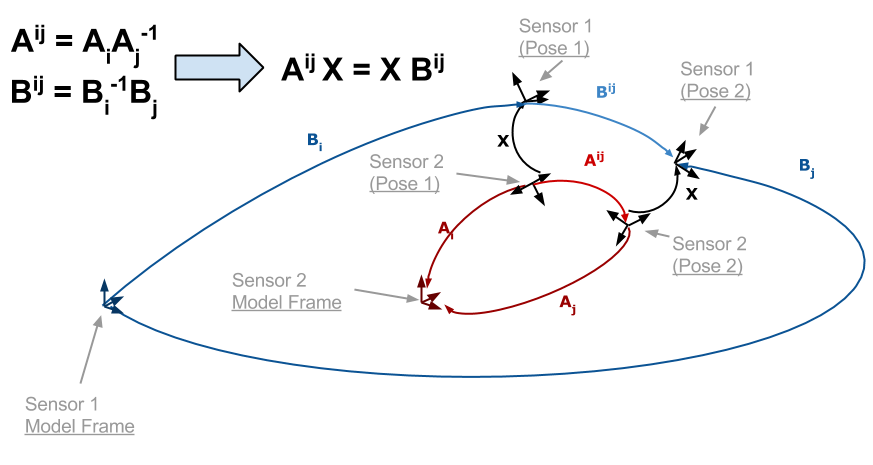
\includegraphics[width=3.3in]{figure/AX=XB(ASME)_v1}
\centering
\caption{The AX=XB Sensor Calibration Formulation {\color{red} Can be replaced with some humanoid robot picture}}
\label{AXXBfig}
\end{figure}

Performing the matrix multiplication of homogeneous transformations in Eq.(\ref{mainaxxb}) and separating out the rotational and translational parts results in two equations of the form:
\begin{equation}
R_A R_X = R_X R_B {\rm \,\,\,\,\, and \,\,\,\,\,} R_A {\bf t}_X + {\bf t}_A = R_X {\bf t}_B + {\bf t}_X.
\label{axxb}
\end{equation}
The strategy to solve Eq.(\ref{mainaxxb}) would appear to reduce to first solving the part of Eq.(\ref{axxb}) with only rotation and then rearranging the second equation so as to find acceptable values of ${\bf t}_X$: $ (R_A - \mathbb{I}_{3}) {\bf t}_X = R_X {\bf t}_B - {\bf t}_A. $ However, there are some problems with this naive approach. As pointed out in \cite{park1994robot,shiu1989calibration}, in nondegenerate cases, there is a one-parameter set of solutions to the first part in Eq.(\ref{axxb}), and the matrix $R_A - \mathbb{I}_{3}$ in general has a rank of $2$. Hence, there are two unspecified degrees of freedom to the
problem, and it cannot be solved uniquely unless additional measurements are taken.

However, if there is sensor error, then it may not be possible to find compatible pairs that reproduce the exact value of $X$. For this reason, minimization approaches are often taken where for $n>2$ a cost function:
\begin{equation}
C(X) = \sum_{i=1}^{n} w_i \, d^2(A_i X,X B_i)
\label{mainaxxb2}
\end{equation}
is computed for some distance metric $d(\cdot,\cdot)$ on $SE(3)$ and $\{w_i\}$ is a set of weights which can be taken to be a partition of unity. 

%A wide variety of such metrics are discussed in \cite{axxb13} that have the useful property of left-invariance, $d(H_0 H_1, H_0 H_2) = d(H_1, H_2)$ for any $H_0, H_1, H_2 \in SE(3)$.
%
%
%Perhaps the simplest of the left-invariant ones is based on the weighted Frobenius norm
%$$ d^2(H_1,H_2) = \|H_1 - H_2\|_{W}^{2} = {\rm trace}[(H_1 - H_2)W(H_1 - H_2)^T] $$
%where $W$ is a matrix that weights rotations and translations appropriately, as described in \cite{axxb13}.
%The sets of pairs $(A_i,B_i)$ for $i=1,2...,n$ is chosen such
%that the set $\{A_i\}$ is spread out over a variety of positions and orientations, and likewise for $\{B_i\}$, so that the
%resulting $X$ is robust to measurement errors. 
The paper is organized as follows. In section 3, we give a detailed review of the existing methods that solve $AX=XB$ problem using $\{A_{i}, B_{i}\}$ pairs with correspondence. The notations in the literature are not consistent and we tried our best to standardize the notations across all the reviewed methods here so that readers can have a straight forward and consistent view of the methods and their relationships. All these methods are able to solve for both the noisy and no noise case. Some approaches are preferable under certain circumstance and their advantages and disadvantages are also highlighted. In section 4, numerical simulations are performed on the selected methods and further conclusions are given based on the results of the simulation. In section 5, a new method called the batch method is presented which does not need a priori knowledge of the correspondence between the sets of measurements $A = \{A_{i}\}$ and $B = \{B_{i}\}$.   

\section{EXISTING SOLUTION METHODS}
 
The problem of solving (\ref{mainaxxb}) for $X$ when multiple corresponding pairs of $A$s and $B$s are presented has a history that goes back more than a quarter of a century
\cite{arun,chou1991finding, park1994robot,shiu1989calibration}, with the earliest proposed by Tsai \cite{tsai1989new} and Shiu \cite{shiu1989calibration}, and applications involving this problem remain active today \cite{dong,kim,dai}. Shah \cite{shah2012overview} overviewed several different AX = XB methods qualitatively, which include but are not limited to the Shiu method, the Lie Group method, the quaternion method, the dual quaternion method, and the Kronecker method. Several new methods emerged recently such as the convex optimization method \cite{zhao2011hand}, the global polynomial optimization method \cite{heller2014hand}, and the gradient descent method \cite{ackerman2014online} etc.
In order to better compare the existing multiple AX = XB methods, we standardize the notations and provide numerical simulations of the above methods. All of the methods mentioned in this section assumes strict correspondence between $A_{i}$ and $B_{i}$.

\begin{comment}
Decompose the 
\begin{equation}
AX = XB,
\label{AXXB}
\end{equation}
decompose Eq.(\ref{AXXB}) into the rotation component and the translation component: 
\begin{equation}
R_{A}R_{X} = R_{X}R_{B}
\label{Rotation}
\end{equation}
\begin{equation}
(R_{A} - I)\ttt_{x} = R_{X}\ttt_{B} - \ttt_{A}
\label{Translation}
\end{equation}
\end{comment}

\subsection{Shiu and Ahmad }
The Shiu and Ahmad method\cite{shiu1989calibration} uses two data pairs $(A_{i}, B_{i})$ to solve for X. The necessary condition for the uniqueness of X is that the rotation axes of $R_{A_1}$ and $R_{A_2}$ are neither parallel nor anti-parallel, and the angles of rotation are neither 0 nor $\pi$. Though this method shows the tolerance of noise to a certain level, it is specifically designed to solve for the case where only two sets of $(A, B)$ are given. 
The rotation matrix $R_{X}$ is solved for first and the translation is obtained using least square technique given known $R_{X}$.\\

The closed form expression for $R_{X}$ is:
\begin{equation}
R_{X} = e^{\tilde{\nn}_{A}\beta}R_{X_{P}}
\label{RotationCheng}
\end{equation}
where 
\begin{center}
$R_{X_{p}} =  e^{\tilde{\nn}_{X}\theta_{X}}$\\
$\nn_{X} = \nn_{B} \times \nn_{A}$\\
$\theta_{X} = \rm atan2(|\nn_{B} \times \nn_{A}|,\nn_{B} \cdot \nn_{A})$\\
\end{center}
and $\beta$ is an arbitrary angle. Given a vector $\nn = \left( n_{1}, n_{2}, n_{3} \right)^{T} \in \mathbb{R}^{3}$, $\tilde{\nn}$ is a skew-symmetric matrix defined as below:\\
\begin{equation}
\tilde{\nn}
=
\begin{pmatrix}
0 & -n_{3} & n_{2} \\
n_{3} & 0 & -n_{1} \\
-n_{2} & n_{1} & 0
\end{pmatrix}.
\end{equation}

Equation (\ref{RotationCheng}) shows that $R_{x}$ has one degree of freedom which is determined by the angle $\beta$. Therefore, two relative arm motions are needed to generate two $(A_{i}, B_{i})$ in order to calculate the unique solution of $X$. Given two pairs of $A$s and $B$s, we have two equations as:
\begin{equation}
\begin{array}{lr}
A_{1}X = XB_{1} \\
A_{2}X = XB_{2}.
\end{array}
\end{equation}
Instead of giving a closed-form solution, $R_{X}$ is calculated by solving for $\beta$ in Eq.(\ref{CYD}), which is formulated by equating two Eq.(\ref{RotationCheng}) that are obtained by $(A_{1}, B_{1})$ and $(A_{2}, B_{2})$:
\begin{equation}
CY = D.
\label{CYD}
%$${\color{red}(Detailed description of C and D?)}$$
\end{equation}
In Eq.(\ref{CYD}), $Y = \big( \; \cos(\beta_{1}),\; \sin(\beta_{1}), \; \cos(\beta_{2}),\; 	\sin(\beta_{2}) \;\big)^{T}$,  $C \in \mathbb{R}^{9 \times 4}$ and $D \in \mathbb{R}^{9 \times 1}$ are determined by $\nn_{A_{1}}$,$\nn_{B_{1}}$, $\nn_{A_{2}}$ and $\nn_{B_{2}}$, and the explicit expressions are given in Eq.(44) of \cite{shiu1989calibration}.\\
 Similarly, with kwown $R_{X}$, $\ttt_{x}$ can be calculated using the least square method:
\begin{equation}
\bigg(\begin{array}{lr}
R_{A_{1}} - \mathbb{I}_{3} \\
R_{A_{2}} - \mathbb{I}_{3}
\end{array}\bigg)\ttt_{X}=
\bigg(\begin{array}{lr}
R_{X}\ttt_{B_{1}} - \ttt_{A_{1}}\\
R_{X}\ttt_{B_{2}} - \ttt_{A_{2}}
\end{array}
\bigg).
\label{trans}
\end{equation}


However, the method proposed here is constrained by two uniqueness conditions of solution, and the author fails to give an explicit closed-form solution of X (neither rotation part $R_{X}$ or translation part $\ttt_{X}$) based on two pairs of $(A_{i},B_{i})$.

\subsection{Lie Group Method }
The Lie Group method \cite{park1994robot} is the first method to solve the AX = XB problem from the perspective of Lie group. It uses the axes of rotation of $A_{i}$ and $B_{i}$ to construct $R_{X}$ and gives both the closed form solution for the no-noise case and the numerical solution for multiple noisy $(A_{i}, B_{i})$ pairs.
\subsubsection{Closed Form Solution with Two Exact Pairs}
The closed-form solution for $R_{X}$ is as follows:
\begin{equation}
R_{X} = \mathcal{A}\mathcal{B}^{-1}
\label{Lie_Rotation}
\end{equation}
where\\

\begin{center}
$\mathcal{A} = (\nn_{A_{1}}, \nn_{A_{2}}, \nn_{A_{1}} \times \nn_{A_{2}})$\\
 $\mathcal{B} = (\nn_{B_{1}}, \nn_{B_{2}}, \nn_{B_{1}} \times \nn_{B_{2}})$\\
$\tilde{\nn}_{A_{1}} = \log(R_{A_{i}})/||(\log R_{A_{i}})^{\vee}||$\\
$\tilde{\nn}_{B_{1}} = \log(R_{B_{i}})/||(\log R_{B_{i}})^{\vee}||$.
\end{center}
The solution for $\ttt_{X}$ can be obtained by Eq.(\ref{trans}) following the same procedure.\\
\begin{comment}
\begin{equation}
\bigg(\begin{array}{lr}
R_{A_{1}} - I \\
R_{A_{2}} - I
\end{array}\bigg)\ttt_{X}=
\bigg(\begin{array}{lr}
R_{X}\ttt_{B_{1}} - \ttt_{A_{1}}\\
R_{X}\ttt_{B_{2}} - \ttt_{A_{2}}
\end{array}
\bigg)
\label{Lie_Translation}
\end{equation}
\end{comment}

\subsubsection{Estimation of X Using Multiple Pairs with Noise}
When there are multiple pairs of $(A_{i}, B_{i})$ with noise, rotation matrix $R_{X}$ is solved for first and then translation vector $\ttt_{x}$ is obtained using least square method given known $R_{X}$. The closed form expression for $R_{X}$ is as follows:
\begin{equation}
R_{X} = (M^{T}M)^{-\frac{1}{2}}M^{T}
\end{equation}
where \\
\begin{center}
$M = \mathlarger{\sum{\nn_{B_{i}} \nn_{A_{i}}^{T}}}$.
\end{center}
Note that $i \geq 3$ is a necessary condition for $M$ to be a non-singular matrix, but it doesn't guarantee $M$ to be nonsingular. Theoretically, the Lie group method is more likely to fail when the number of data pairs is small while in real application, this is barely seen as long as the data pairs are not specially chosen. Given known $R_{X}$, $\ttt_{X}$ can be calculated using the least square method as shown in Eq.(\ref{t_least}):

\begin{equation}
\ttt_{x} = (C^{T}C)^{-1}C^{T}d
\label{t_least}
\end{equation}
where\\

\begin{center}
$\begin{array}{lr}
C = \begin{pmatrix}
\mathbb{I}_{3} - R_{{A_{1}}}\\
\mathbb{I}_{3} - R_{{A_{2}}}\\
.\\
.\\
.\\
\mathbb{I}_{3} - R_{{A_{n}}}\\
\end{pmatrix}
\; \; 
& \; \;
d = \begin{pmatrix}
\ttt_{A_{1}} - R_{X}\ttt_{B_{1}}\\
\ttt_{A_{2}} - R_{X}\ttt_{B_{2}}\\.\\
.\\
.\\
\ttt_{A_{n}} - R_{X}\ttt_{B_{n}}\\\end{pmatrix} 
\end{array}$.
\end{center}


\subsection{Quaternion Method }
The Quaternion Method proposed by Chou \cite{chou1991finding} uses normalized quaternions to transform the rotation parts of $A_{i}X = XB_{i}$ (i = 1,2) into two linear systems. Then singular value decomposition method is performed to obtain a closed form solution of $R_{X}$. In order to estimate $X$ given multiple pairs of $(A_{i}, B_{i})$ with noise, Horaud and Dornaika \cite{horaud1995hand} cast the problem into a nonlinear optimization one. Two different approaches are discussed: (1) estimate the rotation matrix $R_{X}$ by minimizing an objective function, and solve for the translation $\ttt_{X}$ using least square method separately and (2) estimate $R_{X}$ and $\ttt_{X}$ simultaneously by minimizing an objective function that incorporates the information of both rotation and translation. Method (2) is a nonlinear optimization problem which requires an initial guess. In this section, we introduce only the first approach, and the corresponding numerical simulation will be given in section 4.
\subsubsection{Closed Form Solution with Two Exact Pairs}
First, the rotation equation in Eq.(\ref{axxb}) is transformed into the equation of quaternion multiplication as below:
\begin{equation}
R_{A}R_{X} = R_{X}R_{B} 
\; \;
\Leftrightarrow
\; \;
q_{A}\odot q_{X} = q_{X}\odot q_{B}
\label{Quaternion}
\end{equation} 
where $q_{A}$, $q_{B}$ and $q_{X}$ are
unit quaternions that represent the rotation parts of matrices $A$, $B$ and $X$, and $\odot$ denotes the  quaternion multiplication.\\
Given two quaternions $q_{\alpha} = \left( \alpha_{0}, \alpha_{1}, \alpha_{2},\alpha_{3} \right)^{T} = \left( \alpha_{0}, \bf{\alpha}^{T} \right)^{T}$ and $q_{\beta} = \left( \beta_{0}, \beta_{1}, \beta_{2},\beta_{3} \right)^{T} = \left(\beta_{0}, \bf{\beta}^{T} \right)^{T}$, the quaternion multiplication $\odot$ is defined as:
\begin{equation}
q_{\alpha}\odot q_{\beta} = 
\left(
\begin{matrix}
\alpha_{0} \beta_{0} - \bf{\alpha}^{T}\bf{\beta}\\
\beta_{0}\bf{\alpha} + \alpha_{0}\bf{\beta} + \bf{\tilde{\alpha}\beta}
\end{matrix}
\right).
\end{equation}
$\alpha_{0}$ is the scalar component and $\bf{\alpha}$ is the vector component of the quaternion $q_{\alpha}$.
In order to solve for $q_{X}$, the quaternion equation is transformed as
\begin{equation}
E\qq_{X} = \bf 0
\end{equation}
where $E \in \mathbb{R}^{4 \times 4}$ is obtained by grouping $q_{A}$ and $q_{B}$ together, and $\qq_{X} \in \mathbb{R}^4$ is the vector representation of the unit quaternion ${q_X}$.\\

{\color{blue}
For the unit quaternion representing the rotation part of $X$, the resulting expression is: 
\begin{equation}
\qq_{X} = V_{2}\bf y_{2}
\label{QuaternionUnit}
\end{equation}
To obtain $V_{2}$ and $y_{2}$, $E$ is first written as $E =  \sin(\theta_{A|B}/2)M$ with $\theta_{A|B} = \theta_{A} = \theta_{B}$, which is the constraint that corresponding $A$ and $B$ should have the same angle of rotation resulted from the equation AX = XB. Then the singular value decomposition of $M$ is computed as $M = U\Sigma V^{T}$ with $V = (V_{1}, V_{2})$,  $V_{1} \in \mathbb{R}^{4 \times 2}$ and $V_{2} \in \mathbb{R}^{4 \times 2}$. Vector ${\bf y_{2}}$ is obtained by calculating ${\bf y} =  V^{T}\qq_{x}$ where $\bf y = (\bf y^{T}_{1},\bf y^{T}_{2} )^{T}$, ${\bf y_{1}} \in \mathbb{R}^{2 \times 1}$ and ${\bf y_{2}} \in \mathbb{R}^{2 \times 1}$.\\

\begin{center}
$\begin{array}{lcl}
E & = & \sin(\theta_{A|B}/2)M\\
M & = & U\Sigma V^{T}\\
V & = & (V_{1}, V_{2})\\
\bf y & = & V^{T}\qq_{x}\\
\bf y & = & (\bf y^{T}_{1},\bf y^{T}_{2} )^{T}
\end{array}$
\end{center}
}
The translation vector $\ttt_{x}$ satisfies the following equation:
%{\color{red} write equation of $\ttt_{x}$ in a more concise form by substituting c = (A-I)}
%\begin{equation}
%\ttt_{x} = {\bf \nn_{A}} z - \frac{1}{2}\bigg( \cot(\frac{\theta_{A}}{2})\hat{\nn}_{A} + I %\bigg){\bf c}
%\end{equation}
\begin{equation}
\left(\cot(\dfrac{\theta_{A}}{2})\hat{\nn}_{A}(R_{A}-\mathbb{I}_{3})+ R_{A} + \mathbb{I}_{3}\right)\ttt_{x} = \nn_{A}z
\label{QuaternionTranslation} 
\end{equation}
%\begin{equation}
%{\bf c = (R_{A} - I)\ttt_{x}} \;\; \text{  and  } \;\; z \in \mathbb{R} \text{  is arbitrary} 
%\label{QuaternionTranslation}
%\end{equation}
where $z \in \mathbb{R}$ is arbitrary. A unique solution can be calculated using Eq.(\ref{QuaternionUnit}) and Eq.(\ref{QuaternionTranslation}) given two pairs of $(A_{i}, B_{i})$.

\subsubsection{Estimation of X Using Multiple Pairs With Noise} 
In the case where there are n pairs of $(A_{i}, B_{i})$, the problem of recovering $R_{X}$ is converted into minimizing an error objective function as in Eq.(\ref{ErrorQuaternion}):
\begin{equation}
\begin{array}{c}
f(R_{X})
= \sum_{i = 1}^{n}||{n_{A_{i}} - q_{X} \odot n_{B{i}} \odot \bar{q}_{X}}||^{2} \\
\\ 
= {\qq_{X}}^{T}\tilde{K}{\qq_{X}}
\end{array}
\label{ErrorQuaternion} 
\end{equation}
where $n_{A_{i}} = \left(0, {\nn_{A_{i}}}^{T}\right)^{T}$ and $n_{B_{i}} = \left(0, {\nn_{B_{i}}}^{T}\right)^{T}$. $\tilde{K} = \sum_{i = 1}^{n}\tilde{K_{i}}$ and $\tilde{K_{i}} \in \mathbb{R}^{4 \times 4}$ is a symmetric positive definite matrix determined by $\nn_{A_{i}}$ and $\nn_{B_{i}}$; $\bar{q}_{X}$ is the conjugate of ${q}_{X}$ where $q_{X} \odot \bar{q}_{X} = 1$.\\
To minimize  Eq.(\ref{ErrorQuaternion}) under the constraint that $\qq_{X}$ is unit quaternion, the Lagrangian multiplier is introduced in Eq.(\ref{ErrorLagrangeMultiplier}) as:
\begin{equation}
\min_{q} f = \min_{q}({\qq_{X}}^{T}\tilde{K}{\qq_{X}} + \lambda(1 - {\qq_{X}}^{T}{\qq_{X}})).
\label{ErrorLagrangeMultiplier}
\end{equation}
Differentiate the error function with respect to $\qq_{X}$, the 1st order necessary optimality condition is obtained as: 
\begin{equation}
\tilde{K}\qq_{X} = \lambda \qq_{X}.
\label{QuaternionEig}
\end{equation}
A closed form solution can be easily found, and the unit quaternion $\qq_{X}$ that minimizes $f$ is the eigenvector of $\tilde{K}$ associated with its smallest positive eigenvalue. After recovering $\qq_{X}$ (or equivalently $R_{X}$), $\ttt_{X}$ can be recovered using the least square technique as introduced in previous methods.




\subsection{Dual Quaternion Method }
The dual quaternion method \cite{daniilidis1999hand} treats the rotation and translation parts of the matrix X in a unified way and facilitates a new simultaneous solution of X using the singular value decomposition method. To begin with, Eq.(\ref{mainaxxb}) is transformed into an equation in dual quaternion form as follows:
\begin{equation}
AX = XB 
\; \;
\Leftrightarrow
\; \;
\check{a} = \check{q}_{X}\hat{\odot}\check{b}\hat{\odot}\bar{\check{q}}_{X}
\label{DualQuaternion}
\end{equation}
where $\check{a}$, $\check{b}$ and $\check{q}$ are the dual quaternions that represent matrices $A$, $B$ and $X$, and $\bar{\check{q}}$ is the conjugate of $\check{q}$.\\
The dual quaternion that corresponds to a 4 by 4 rigid transformation matrix is defined as follows:
\begin{equation}
\check{q}_{X} =
\Bigg( 
\begin{array}{c}
\cos(\frac{\theta + \epsilon d}{2})\\
\sin(\frac{\theta + \epsilon d}{2})({\bf l} + \epsilon {\bf m})
\end{array}
\Bigg)
\label{dual_screw}
\end{equation}
where
$\theta$, $d$, ${\bf l}$ and ${\bf m}$ are screw parameters and ${\epsilon}^{2} = 0$. $\theta$ is the rotation angle, $d$ is the pitch, $\vec{\bf l}$ is the direction of the screw, and ${\bf m} = {\bf p} \times {\bf l}$ is the line moment where ${\bf p}$ is a point on the line. The six tuple $({\bf l}, {\bf m})$ defines a line in 3-D space. Furthermore, by expanding the dual terms in $\check{q}_{X}$, Eq.(\ref{dual_screw}) can also be written as:
\begin{equation}
\check{q}_{X} = q_{X} + \epsilon {q}^{\prime}_{X}.
\end{equation} 
Both $q$ and $q^{\prime}$ are quaternions satisfying the following constraints:
\begin{equation}
{\bf q}^{T}_{X}{\bf q}_{X} = 1 \; \; \text{and} \;
\; {\bf q}^{T}_{X}{\bf q}^{\prime}_{X} = 0.
\end{equation}
Similar to Section 3, ${\bf q}_{X}$ and ${\bf q}^{\prime}_{X}$ are the vector representations of $q_{X}$ and $q^{\prime}_{X}$.
Then equation $A_{i}X = XB_{i}$ can be converted into the form as below:

\begin{equation}
S_{i}
\bigg(
\begin{array}{c}
{\bf q}_{X}\\
{\bf q}^{\prime}_{X}

\end{array}
\bigg) = \bf 0
\end{equation} 
where
\begin{equation}
S_{i} = 
\bigg(
\begin{array}{cccc}

{\aaa} - {\bbb} & \; ({\aaa} + {\bbb})^{\wedge} & \; \bf 0_{3\times 1} & \bf 0_{3\times 3}\\

{\aaa}^{\prime} - {\bbb}^{\prime} & ({{\aaa}^{\prime} + {\bbb}^{\prime}})^{\wedge} & {\aaa} - {\bbb} & ({\aaa} + {\bbb})^{\wedge} 

\end{array}
\bigg) \in \mathbb{R}^{6 \times 8}.
\end{equation}
${\aaa}^{\prime} = \dfrac{1}{2}{\ttt}_{X} \times {\aaa}$ and $\aaa$ is the vector part of $q_{X}$.
After concatenating $S_{i}$, matrix $T$ can be obtained and used to solve for $X$.
\begin{equation}
T = \big( \; \; S_{1}^{T} \; S_{2}^{T} \; \; ... \; \; S_{n}^{T} \; \; \big)^{T}
\end{equation}
By calculating the singular value decomposition on $T = U\Sigma V^{T}$, the dual quaternion for matrix X can be expressed as the linear combination of the last two right-singular vectors (${\bf v_{7}}$, ${\bf v_{8}}$) of matrix $T$ , which are just the last two columns of matrix $V$, as shown in Eq.(\ref{dq_closed}): 
\begin{equation}
\bigg(
\begin{array}{c}
{\bf q}_{X}\\
{\bf q}^{\prime}_{X}
\end{array}
\bigg) = 
\lambda_{1}{\bf v_{7}} + \lambda_{2}{\bf v_{8}} \in \mathbb{R}^{8} \; \;
\text{where} \; \; \lambda_{1}, \lambda_{2} \in \mathbb{R}.
\label{dq_closed}
\end{equation} 

Different from the quaternion method (\ref{Quaternion}), the dual quaternion method solves the rotational part and translational part in a united way, and it contains all the information to reconstruct matrix $X$. Despite the advantages of the dual quaternion method, it has the drawback of having to filter the data pairs to provide inappropriate solutions when there is noise on $A_{i}$ and $B_{i}$.

\subsection{\color{blue} Kronecker Product Method }
Inspired by the well known Sylvester equation ( $AX + XB = C$ ) in linear systems, the Kronecker method converts  Eq.(\ref{mainaxxb}) into the form of Kronecker products \cite{andreff1999line} as in Eq.(\ref{KroneckerMethod}):
\begin{equation}
\begin{split}
AX = XB  \Leftrightarrow\\
\Bigg(
\begin{array}{cc}
\mathbb{I}_{9} - R_{B} \otimes R_{A} \; & \; 0_{9 \times 3}\\
\ttt_{B}^{T} \otimes \mathbb{I}_{3} & \mathbb{I}_{3} - R_{A}
\end{array}
\Bigg) 
\Bigg(
\begin{array}{c}
vec(R_{X})\\
\ttt_{X}
\end{array}
\Bigg) =
\Bigg(
\begin{array}{c}
0_{9}\\
\ttt_{A}
\end{array}
\Bigg).
\end{split}
\label{KroneckerMethod}
\end{equation}
%where the symbol $\otimes$ denotes the Kronecker product. The $vec$ operator was introduced in \cite{neudecker1969note} and it's used to reorder the $m \times n$ components of a matrix $M_{m \times n}$ into a $mn$ vector $vec(M_{m \times n})$.\\
Given multiple pairs of $A$s and $B$s with noise, the Kroneker product is reformulated as Eq.(\ref{KroneckerRotation}) and Eq.(\ref{KroneckerTrans}):
\begin{equation}
\left(
\begin{array}{c}
\mathbb{I}_{9} - R_{B_{1}} \otimes R_{A_{1}}\\
\mathbb{I}_{9} - R_{B_{2}} \otimes R_{A_{2}}\\
\vdots\\
I_{9} - R_{B_{n}} \otimes R_{A_{n}}
\end{array}
\right) 
vec(R_{X})
 = {\bf{0}}_{9 n \times 1},
\label{KroneckerRotation}
\end{equation}
\begin{equation}
\left(
\begin{array}{c}
\mathbb{I}_{3} - R_{A_{1}} \\
\mathbb{I}_{3} - R_{A_{2}} \\
\vdots\\
\mathbb{I}_{3} - R_{A_{n}}
\end{array}
\right) 
{\ttt_{X}}
 = 
\left( 
\begin{array}{c}
{\bf{t}}_{A_{1}} - R_{X}{\bf{t}}_{B_{1}}\\
{\bf{t}}_{A_{2}} - R_{X}{\bf{t}}_{B_{2}}\\
\vdots\\
{\bf{t}}_{A_{n}} - R_{X}{\bf{t}}_{B_{n}}\\
\end{array}
\right).
\label{KroneckerTrans}
\end{equation}
{\color{blue}
Orthogonalization is implemented on $R_{X}$ to make it a rotation matrix. \\
\begin{equation}
R_{X_{e}} = R_{X}(R_{X}^{T}R_{X})^{-1/2}
\label{Orthogonolization}
\end{equation}
\cite{horn1986robot}
where $R_{X_{e}}$ denotes the orthogonalized $R_{X}$.\\
The orthogonalized matrix $R_{X_{e}}$ is further normalized as in Eq.(\ref{kron_normal}), then the rotation matrix $R_{X} \in SO(3)$ is obtained. 
\begin{equation}
R_{X_{n}} = \dfrac{sign(\textrm{det}(R_{X_{e}}))}{{|\textrm{det}(R_{X_{e}})|}^{\tfrac{1}{3}}}R_{X_{e}}
\label{kron_normal}
\end{equation}
where $R_{X_{n}}$ is the normalized matrix of $R_{X_{e}}$.
After obtaining the estimation of $R_{X}$, least square method is implemented on Eq.(\ref{KroneckerTrans}) to recover the value of $\ttt_{X}$.  
}
\subsection{Global Polynomial Optimization}
{\color{red}To be added or not?}

\subsection{Convex Optimization}
{\color{red}To be added or not?}

\subsection{Gradient Descent Method}
All the methods mentioned above are only able to solve for matrix $X$ offline, which means $\{A_{i}, B_{i}\}$ data pairs should be fully collected before being put into the algorithm. The gradient descent method \cite{ackerman2014online} is an online sensor calibration method which uses a gradient descent optimization on the Euclidean group (SE(3)) given an appropriate cost function. 

In the first place, define $\mathcal{X} \in se(3)$ as the Lie algebra corresponding to $G = SE(3)$, and let $f:G \rightarrow \mathbb{R}$ be an analytic function and $g \in G$. As defined in \cite{myoldbook}, the concept of directional derivatives in $\mathbb{R}^{n}$ is extended to functions on a Lie group as:
\begin{equation}
\left.(\hat{\mathcal{X}}^{r}f)(g)\doteq \dfrac{d}{dt}f(g\circ \text{exp}(t\mathcal{X}))\right\vert_{t=0}.
\label{r_lie_d}
\end{equation}
Note that $t$ is just a scalar, while $\ttt$ represents the translation part of a homogeneous transformation.
Eq.(\ref{r_lie_d}) is the ``right'' Lie derivative and the ``left'' Lie derivative is defined in a similar form. A gradient on $SE(3)$ can be defined using the right Lie derivative with the ``natural'' basis of Lie algebra $\{E_{i}\}$ where $i = 1,2,...,6$. Therefore, the gradient of the function on Lie group $f(g)$ is as follows:
\begin{equation}
\nabla f(g)= \left( 
\begin{matrix}
\frac{d}{dt}\left.f(g\circ \text{exp}(tE_{1}))\right\vert _{t=0} \\
\frac{d}{dt}\left.f(g\circ \text{exp}(tE_{2}))\right\vert _{t=0} \\
\vdots \\
\frac{d}{dt}\left.f(g\circ \text{exp}(tE_{6}))\right\vert _{t=0}.
\end{matrix}
\right)
\end{equation}

In order to update $g$, the rigid boy velocity is introduced where $V^{r}_{g} = g^{-1}\dot{g}$, and the update law is written as below:
\begin{equation}
g_{s+1} = g_{s}\text{exp}(\Delta t V^{r}_{g})
\end{equation}
where $t_{s+1} = t_{s} + \Delta t$ is the discrete time step. To complete the update update law, the rigid body velocity is defined as: 
\begin{equation}
V^{r}_{g} = g^{-1}\dot{g} = -\alpha \widehat{\nabla f(g)}.
\end{equation} 
The cost function can be chosen as:
\begin{equation}
C(X) = \sum_{i=1}^{n}||A_{i}X - XB_{i}||.
\end{equation}

The gradient descent method updates the calibrations parameters online based on new incoming data. The initial guess of $X$ will converge to the true $X$, however, the rate of convergence depends on how ``good'' the initial guesses are.
\section{NUMERICAL SIMULATION AND ERROR COMPARISON}
\label{qianli-numerical}

In this section, we numerically simulated the Lie group method, the Kronecker product method, the quaternion method, and the dual quaternion method in Matlab  to compare the errors in both $R_{X}$ and $t_{x}$ with respect to different noise levels on $\{A_{i}, B_{i}\}$. 

\subsection{Error Metrics and Covariance Matrix}
There are multiple ways to define the errors of rigid body transformation. One approach is to measure the errors of $R_{x}$ and ${\bf t}_{X}$ simultaneously. The other approach is to measure the rotation error and translation error separately. 
\subsubsection{Metrics for Rotation Error}
Various metrics for rotation error have been used in the literature. For one time of simulation, in \cite{tsai1989new} and \cite{horaud1995hand}, the matrix error norm is used as: 
\begin{equation}
E_{rot} \doteq \| R_{X_{true}} - R_{X_{calc}} \|,
\end{equation}
In \cite{daniilidis1999hand} and \cite{andreff1999line}, the quaternionic error norm is used as:
\begin{equation}
E_{rot} \doteq \|{\bf q}_{X_{true}} - {\bf q}_{X_{calc}}\|,
\end{equation}
Another way is to calculate the Frobenius norm of the relative rotation between $X_{true}$ and $X_{calc}$ as:
\begin{equation}
E_{rot} \doteq \|R^{T}_{X_{true}}R_{X_{calc}}\|_{F},
\end{equation} 
We further propose the Lie algebra error for the relative rotation $R^{T}_{X_{true}}R_{X_{calc}}$ as:
\begin{equation} 
E_{rot} \doteq \|\log^{\vee}(R_{X_{true}}^TR_{X_{calc}})\|_{2}.
\label{RotError}
\end{equation}
By using metrics in Lie algebra, it is possible to avoid any weighting biasing that might appear in metrics involving a norm. 

\subsubsection{Metrics for Translation Error and Error Covariance Matrix}
Metrics for translation error are simple because translation lies in the Euclidean space. A common way is to use the relative error in translation to eliminate the influence of the unit:
\begin{equation}
E_{tran} \doteq \dfrac{\|\ttt_{X_{true}}-\ttt_{X_{calc}}\|_{2}}{\|\ttt_{X_{true}}\|_{2}}.
\label{TranError}
\end{equation}
Furthermore, we compared the accuracy of the 4 methods by calculating their error covariance matrices $^e\Sigma$, which is defined as:
\begin{equation}
^e\Sigma \doteq \sum_{i = 1}^{n}K_{i}K_{i}^{T} \in \mathbb{R}^{6 \times 6}.
\end{equation}
where $K_{i} = \log^{\vee}(A_{i}) - Ad(X_{calc})\log^{\vee}(B_{i})$.
%\begin{figure}[h]
%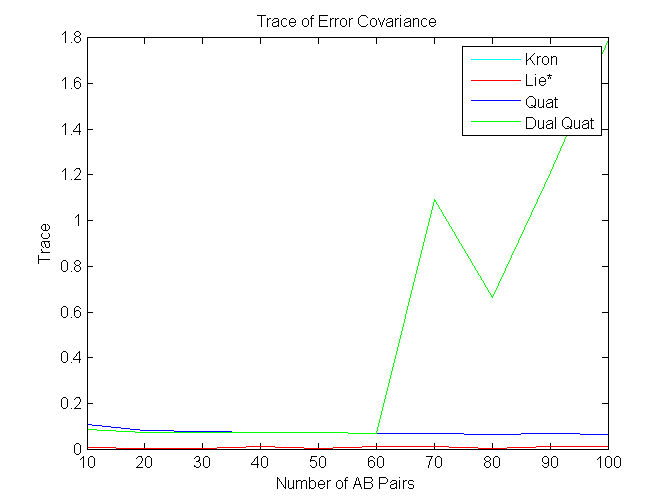
\includegraphics[scale=0.5]{figure/traceCov}
%\centering
%\label{fig:Trace}
%\caption{Trace of the Error Covariance Matrix}
%\end{figure}
The error covariance matrix $^e\Sigma$ can provide information about the variances of the independent and correlated error on each basis of Lie algebra. 

\subsection{$\{A_{i}, B_{i}\}$ Pairs Generation}
There are various ways of generating noisy $\{A_{i},B_{i}\}$ pairs and different data sets can cause certain methods to perform badly or even to crash. To simulate different $AX=XB$ solvers with synchronous noisy $\{A_{i},B_{i}\}$ pairs, we first generate $B_{i}$ by randomly sampling the Lie algebra of matrix $B_{i}$, and then recover $B_{i}$ using the matrix exponential as shown below:
\begin{equation}
B_{i} = \exp \left(
\begin{array}{ccc}
\Omega_{i}  & & {\bf v_{i}}  \\ \\
{\bf 0}^T & & 0 \end{array}
\right).
\end{equation} 
Next, the noisy $A_{i}$ is obtained by $A_{i}= ^1\hspace{-0.05in}X_{i}\,\,B_i\,\,^2X_{i}^{-1}$ where $^1X_{i}$ and $^2X_{i}$ are calculated by applying small disturbances on the ground truth $X_{true}$: 
\begin{equation}
^mX_{i} = X_{true}\exp \left(
\begin{array}{ccc}
^m\Omega_{X_{i}}  & & ^m{\bf v}_{X_{i}}  \\ \\
{\bf 0}^T & & 0 \end{array}
\right)
\; \;
\text{where} \; \; m = 1,2
\label{X_disturb}
\end{equation}
where $\omega_{X_{i}}$ and ${\bf v}_{X_{i}}$ are drawn from independent Gaussian distributions. In order to test the sensitivity to different noise levels for each $AX=XB$ solver, we choose the mean of $\left(\omega_{X_{i}}^{T}, {\bf v}_{X_{i}}^{T}\right)^{T}$ to be ${\bf 0}_{6 \times 1}$ and its covariance matrix to be $\Sigma_{X_{i}} = \sigma^{2} \mathbb{I}_{6}$ with $\sigma$ ranging from 0 to 0.1.


%-------------------------------------------------
\subsection{Numerical Simulation Result}
The numerical simulation results are presented in Fig.\ref{roterror}, Fig.\ref{transerror}, and Fig.\ref{traceerror}. Figure \ref{roterror} shows that as the noise level $\sigma$ increases, Lie group method shows the least increase in rotation error, while the dual quaternion method's increase in the rotation error is the largest. The rotation errors of the Kronecker method (light blue line) and the quaternion method (dark blue line) are pretty close and they are even closer in terms of translational error (figure \ref{transerror}).

\begin{figure}[h]
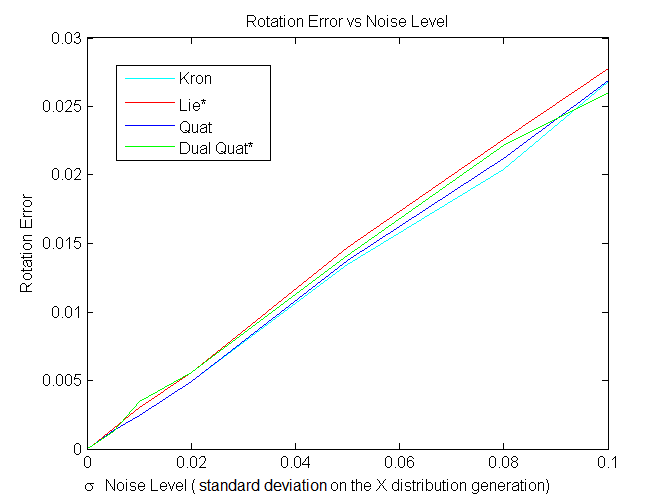
\includegraphics[width=3.3in]{figure/rotErrorRand}
\centering
\caption{Rotation Error v.s. Noise Level using Lie algebra Error Metric }
\label{roterror}
\end{figure}

{\color{blue} Lie$^{\star}$ is an improved version of the original Lie group method where ill-conditioned $\{A_{i},B_{i}\}$ pairs are eliminated solving for the estimated $X$. This is due to the limitation of algorithm that $A_{i}$ or $B_{i}$ whose trace is equal or very close to -1 will cause the singularity of numerical computation. Different ways of generating $\{A_{i},B_{i}\}$ can affect the number of filtered pairs and certain ways can render the Lie group method giving $R_{X}$ with $\det(R_{X}) = -1$.\\

Dual Quat$^{\star}$ also eliminates certain $\{A_{i},B_{i}\}$ pairs by checking the proximity of the scalar parts of the dual quaternions of $A_{i}$ and $B_{i}$ under certain boundary. Similar to the Lie group method, the way of generating $\{A_{i},B_{i}\}$ pairs can affect the number of filtered data, and this will affect the accuracy of the estimated $X$. In addition, certain ways of generating the data pairs can cause the dual quaternion method failing to give a valid result from fixed filtered data pairs. This problem can possibly be solved by extracting a smaller portion of the given $\{A_{i},B_{i}\}$ pairs but this also can degrade the accuracy of the result.  
\begin{figure}[h]
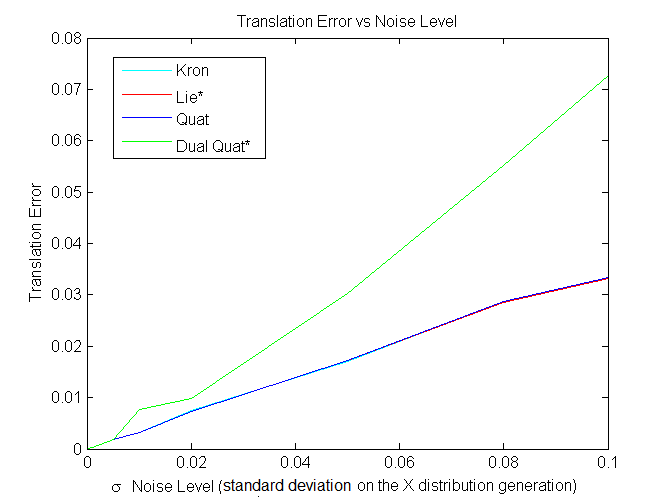
\includegraphics[width=3.3in]{figure/tranErrorRand}
\centering
\caption{Translation Error with Randomly Generated AB Pairs (with the improved Lie and Dual Quaternion methods)}
\label{transerror}
\end{figure}

\begin{figure}[h]
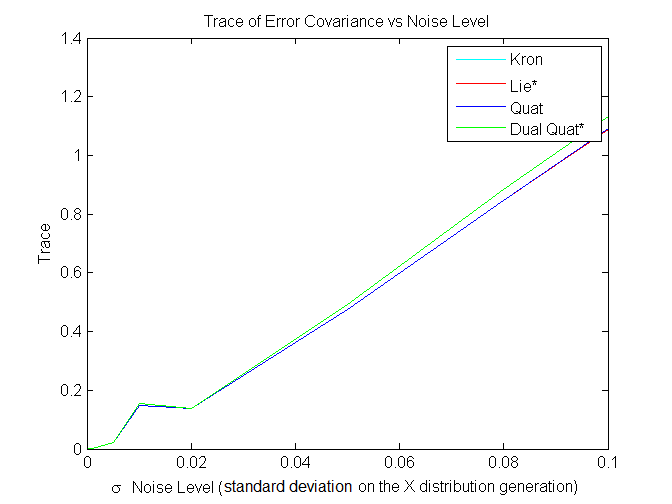
\includegraphics[width=3.3in]{figure/traceCovRand}
\centering
\caption{Trace of the Error Covariance Matrix}
\label{traceerror}
\end{figure}

In general, all of the traditional methods work well with near random Gaussian distributed noisy $\{A_{i},B_{i}\}$ pairs. However, it should be noted that in many applications the information of $\{A_{i},B_{i}\}$ is obtained by moving the calibration sensor along a trajectory. Depending on the specifics of the trajectory, as well as the sample rate along the trajectory, the data may become ill conditioned for these methods.}

A commonality of all the methods in the previous section is that exact knowledge of $\{A_i\}$ and $\{B_j\}$ correspondence is assumed, however, this is not always the case. There are many instances in the literature when the sensor data used in calibration becomes ``unsynchronized''. Different attempts have been implemented to solve this problem, such as time stamping the data, developing dedicated software modules for syncing the data \cite{alexis9}, and analyzing components of the sensor data stream to determine a correlation \cite{darius1}, to varying effects. The solution methodology presented in this paper bypasses these issues altogether without tracking, or recomputing, correspondence. By modeling the set of $A$s and $B$s as probability distributions on $SE(3)$, the data can be taken as an unordered, uncorrelated ``batch" and a solution for $X$ can be generated. Additionally, this new formulation can be expanded to more explicitly model the error in $X$ associated with the noise in $A$s and $B$s. The error can then be minimized to further refine $X$.

In the following section we present a new solution method to the $AX=XB$ formulation that does not require the correspondence to be known between $(A, B)$ pairs.
\section{THE BATCH METHOD (THE NOISE-FREE CASE)}
\label{batchnoisefree}

This section presents new methods to solve for $X$ wherein there does not need to be any priori knowledge of the correspondence between the exact sets of measurements
$A = \{A_i\}$ and $B = \{B_j\}$. In other words, the sets $A$ and $B$ each can be given as unordered ``batches'' without knowing how each $A_i$ matches to a $B_j$.

\subsection{The Batch Method Formulation}
Given a large set of pairs $(A_i,B_i) \in SE(3) \times SE(3)$ for $i =1,...,n$ that exactly satisfy the equation:
\begin{equation} A_i X = X B_i \label{main} \end{equation}
a new algorithm is developed to find $X \in SE(3)$. We address a generalization of the standard problem in which
the sets $A=\{A_i\}$ and $B =\{B_j\}$ are provided with elements written in any order and it is known that a correspondence exists between the elements of these sets such that Eq.(\ref{main}) holds, but we do not know a priori of this correspondence between each $A_i$ and $B_j$.

We begin by defining a Gaussian probability distribution on $SE(3)$ (assuming the norm $\|\Sigma\|$ is small) as
$$ \rho(H; M, \Sigma) = \frac{1}{(2\pi)^3 |\Sigma|^{\half}} e^{-\half F(M^{-1} H)} $$
where $|\Sigma|$ denotes the determinant of $\Sigma$ and
$$ F(H) = [\log^{\vee}(H)]^T \Sigma^{-1} [\log^{\vee}(H)]. $$
When $H$ is parameterized with exponential coordinates, $H = \exp Z$, this means that
$F(\exp Z) = {\bf z}^T \Sigma^{-1}  {\bf z}$ where ${\bf z} = Z^{\vee}$ and
$\rho(\exp Z; \mathbb{I}_4, \Sigma)$ becomes exactly a zero-mean Gaussian distribution on the Lie algebra $se(3)$, with covariance $\Sigma$, that is `lifted up' to the Lie group $SE(3)$. This definition is valid when $\|\Sigma\|$ is small enough that the tails of the distribution decay rapidly enough that the value of $\rho$
becomes negligible before they ``wrap around'' due to the topology of $SE(3)$. 

Using formulations of probability theory on SE(3), we can think of Eq.(\ref{main}) as:
\begin{equation} (\delta_{A_i} * \delta_X)(H) = (\delta_X * \delta_{B_i})(H) \label{mainconv} \end{equation}
where $*$ denotes the convolution of functions on $SE(3)$, as defined in the Appendix.

Whereas the addition (as opposed to multiplication) of homogeneous transformation matrices is nonsensical, the addition of real-valued functions $f_1(H) + f_2(H)$ is a perfectly reasonable operation and since convolution is a linear operation on functions, we can write all $n$ instances of Eq.(\ref{mainconv}) into a single equation of the form
\begin{equation} (f_A * \delta_X)(H) = (\delta_X * f_B)(H) \label{mainconvall} \end{equation}
where $$ f_A(H) = \frac{1}{n} \sum_{i=1}^{n} \delta(A_i^{-1} H) \,\,\, {\rm and} \,\,\, f_B(H) = \frac{1}{n} \sum_{i=1}^{n} \delta(B_i^{-1} H). $$
The above functions can be normalized
to be probability densities:
$$ \int_{SE(3)} f_A(H) dH = \int_{SE(3)} f_B(H) dH = 1. $$
See the Appendix for a review of the properties of integration on $SE(3)$.

Let the mean and covariance of a probability density $f(H)$ be defined by the conditions
\begin{equation} \begin{split} &\int_{SE(3)} \log(M^{-1} H) f(H) dH = \mathbb{O} \,\,\, {\rm and} \,\,\,\\ &\Sigma = \int_{SE(3)} \log^{\vee}(M^{-1} H) [\log^{\vee}(M^{-1} H)]^T  f(H) dH . \end{split}\label{meancovdef} \end{equation}
If $f(H)$ is of the form of $f_A(H)$ given above, then
\begin{equation} \
\begin{split} &\sum_{i=1}^{n} \log(M_A^{-1} A_i) = \mathbb{O} {\rm \,\,\,\,\, and} \\
&\Sigma_A = \frac{1}{n} \sum_{i=1}^{n} \log^{\vee}(M_A^{-1} A_i) [\log^{\vee}(M_A^{-1} A_i)]^T.  \label{datameancovconvdef} \end{split}
\end{equation}

It can be shown that if these quantities are computed for two highly focused functions, $f_1$ and $f_2$, that the same quantities for
the convolution of these functions can be closely approximated as \cite{Wang08}:
\begin{equation}
M_{1*2} = M_1 \, M_2 \,\,\, {\rm and} \,\,\, \Sigma_{1*2} = Ad(M_2^{-1}) \,\Sigma_{1}\, Ad^T(M_2^{-1}) + \Sigma_{2}
\label{meancovconvdef} \end{equation}
where
\begin{equation} 
Ad(H) = \left(\begin{array}{ccc}
R && \mathbb{O} \\
\widehat{{\bf x}} R && R \end{array}\right) 
\label{adjdef} \end{equation}
and $\widehat{{\bf a}}$ is the skew-symmetric matrix such that $\widehat{{\bf a}} {\bf b} = {\bf a} \times {\bf b}$.

The mean of $\delta_X(H)$ is $M_X = X$, and its covariance is the zero matrix.
Therefore, Eq.(\ref{mainconvall}) together with Eq.(\ref{meancovconvdef}) gives two``Batch Method" equations:
\begin{equation}
\boxed{\,
M_A \, X = X \, M_B
\,}
\label{mainmain11} \end{equation}
and
\begin{equation}
\boxed{\,
Ad(X^{-1}) \, \Sigma_{A} \, Ad^T(X^{-1}) = \Sigma_{B}
\,}
\label{mainmain12} \end{equation}

For the problem discussed in this paper, there is no loss of generality in assuming that $\|\Sigma_A\|$ and $\|\Sigma_B\|$
are small because the constraint Eq.(\ref{mainmain12}) is linear
in $\Sigma_A$ and $\Sigma_B$, and if they are not small, they can both be normalized as $\Sigma'_A = \Sigma_A/(\|\Sigma_A\|) $ and likewise
$\Sigma'_B = \Sigma_B/(\|\Sigma_A\|)$. Note that here we have normalized by the same quantity on both sides. We cannot use $\|\Sigma_A\|$ on one side
of the equation and $\|\Sigma_B\|$ on the other because the Frobenius norm is not $Ad$-invariant for $SE(3)$.

Moreover, standard tests from multivariate statistical analysis such as q-q plots can be used to assess whether or not the data are
Gaussian. If they are not, they can be made Gaussian without loss of information or by introducing changes to the original mean and covariance in a simple way.
With $A_i = X B_i X^{-1}$, it follows that $A_i^p = X B_i^p X^{-1}$ for any power $p \in \mathbb{R}$. This means that each measured data point can be
replaced with a continuum of equivalent data points parameterized by $p$. Practically speaking, we can sample $p$ at fractional powers in the range
$p\in [-1,1]$ and introduce multiple instances of samples with a Gaussian weighting that depends on $p$. This would cause the resulting augmented data set
to behave as a Gaussian. But since the mean and covariance would be unchanged, there is no need to implement this thought experiment -- Gaussians can be
used in place of data that are not even Gaussian.

Having said all of this, the following theorem indicates that we do not have to limit the discussion to highly concentrated pdfs.
{\color{red} Double check whether this has been published in previous papers. If not, remove completely; otherwise, briefly mention the idea and remove the detailed equations.}
\begin{theorem} \label{exactthm}
Unlike Eq.(\ref{meancovconvdef}), Eq.(\ref{mainmain11}) and Eq.(\ref{mainmain12}) are exact (rather than approximate) 
expressions that do not depend on the smallness of $\Sigma$ or any assumptions about the form of
the functions $f_A$ or $f_B$. 
\end{theorem}

\begin{proof}
Starting with Eq.(\ref{mainconv}), performing a convolution on the left of both sides of the equation with
$\delta_{X^{-1}}(H)$, and using the associativity of convolution and the properties of delta functions reviewed
in the Appendix, Eq.(\ref{mainconv}) can be replaced with:
$$ (\delta_{X^{-1}} * \delta_{A_i} * \delta_X)(H) = \delta_{B_i}(H), $$
and summing both sides over $i$ and dividing by $n$ gives 
\begin{equation} (\delta_{X^{-1}} * f_A * \delta_X)(H) = f_B(H). \label{deltabothsides} \end{equation}
Let $M_A$ be the mean of $f_A$ and $M_B$ be the mean of $f_B$. 
Again using the properties of the delta function given in the Appendix, and using Eq.(\ref{deltabothsides}), 
$$ \int_{SE(3)} \log({M}_{B}^{-1} H) (\delta_{X^{-1}} * f_A * \delta_{X})(H) dH = $$
$$ \int_{SE(3)} \log({M}_{B}^{-1} H) f_A({X} H {X}^{-1}) dH = \mathbb{O}. $$
Changing variables as $K = {X} H {X}^{-1}$ and using the invariance of integration (also given in the Appendix),
$$ \int_{SE(3)} \log({M}_{B}^{-1} X^{-1} K X) f_A(K) dK = \mathbb{O}. $$
Multiplying on the left by $X$ and right by $X^{-1}$ and using the fact that
$X[\log({M}_{B}^{-1} X^{-1} K X)]X^{-1} = \log(X {M}_{B}^{-1} X^{-1} K)$ gives
$X {M}_{B}^{-1} X^{-1} = M_{A}^{-1}$, which is the same as Eq.(\ref{mainmain11}). The proof for Eq.(\ref{mainmain12}) follows in a similar way.
\end{proof}

The generality of this result, which follows from convolution of one function on either side by a function and a version of itself with inverted argument,
motivates much of the theoretical developments that occur later in the paper. But first, we address how to solve Eq.(\ref{mainmain11}) and Eq.(\ref{mainmain12}) 
for $X$. 

\subsection{A Batch Method Solution}

Starting with Eq.(\ref{mainmain11}), we can identify the solution space of $X$ is a cylinder. Specifically Eq.(\ref{mainmain11}) can be rewritten as:

\begin{equation}
\log^{\vee}(M_A)  = Ad(X) \,\log^{\vee}(M_B).
\label{mainmain1rewrite} \end{equation}

In the case of general $M_A$ and $M_B$ (i.e., not degenerate cases in which the rotation angle\footnote{This angle is computed from the Frobenius norm $\theta_A =\|\half \log R_A\| = \|\half \log R_B\|= \theta_B$.} is outside of the range
$(0,\pi)$, the solution space of all possible $X$s that satisfy this equation is known to be two dimensional.
This can be seen by defining
$$ \log^{\vee}(M) = \left(\begin{array}{c}
\omega \\
{\bf v} \end{array} \right)
=\left(\begin{array}{c}
\theta \, {\bf n} \\
{\bf v} \end{array} \right), $$
where ${\bf \omega} \in \mathbb{R}^3$ and ${\bf v} \in \mathbb{R}^3$ are the elements of the Lie Algebra, and writing the rotation and translation parts of Eq.(\ref{mainmain1rewrite}) separately,
\begin{equation}
{\bf n}_A = R_X {\bf n}_B \hspace{5mm}\mbox{and}
\label{nanb} \end{equation}
\begin{equation}
{\bf v}_A = \theta_B \widehat{\,{\bf t}_X} R_X {\bf n}_B + R_X {\bf v}_B.
\label{vavb} \end{equation}
The first of these equations has a one-dimensional solution space of the form
$R_X = R({\bf n}_A, {\bf n}_B) R({\bf n}_B, \phi)$ where $\phi \in [0,2\pi)$ is free and
$R({\bf n}_A, {\bf n}_B)$ is any rotation matrix that rotates the vector ${\bf n}_B$ into ${\bf n}_A$.
In particular, we can choose
\begin{equation}
R({\bf n}_A, {\bf n}_B)  \,=\,
\II \,+\, \widehat{{\bf n}_B \times {\bf n}_A}
\,+\, \frac{(1- {\bf n}_B \cdot {\bf n}_A)}{\|{\bf n}_B \times {\bf n}_A\|^2} \, \left(\widehat{{\bf n}_B \times {\bf n}_A}\right)^2.
\label{transab}
\end{equation}
The rotation $R({\bf n}_B, \phi)$ is given by Euler's formula:
$$ R({\bf n}_B, \phi) = \II \,+\, \sin \phi \, \widehat{\,{\bf n}_B} \,+\, (1-\cos \phi)\, \left(\widehat{\,{\bf n}_B}\right)^2. $$

Substituting $R_X = R({\bf n}_A, {\bf n}_B) R({\bf n}_B, \phi)$ into Eq.(\ref{vavb}) and rearranging terms, we get:
\begin{equation}
\frac{R({\bf n}_A, {\bf n}_B) R({\bf n}_B, \phi) {\bf v}_B - {\bf v}_A}{\theta_B} = \widehat{\, {\bf n}_A} {\bf t}_X.
\label{transcon} \end{equation}
The skew-symmetric matrix $\widehat{\, {\bf n}_A}$ has a rank of 2, so a free translational degree of freedom exists in ${\bf t}_X$ along the ${\bf n}_A$ direction. ${\bf t}_X$ can thus be described as:
\begin{equation}
{\bf t}_X =  {\bf t}(s) = s \, {\bf n}_A + a \, {\bf m}_A + b \, {\bf m}_A \times {\bf n}_A
\label{transparam} \end{equation}
where $s \in \mathbb{R}$ is a second free parameter, ${\bf m}_A$ and ${\bf m}_A \times {\bf n}_A$ are
defined to be orthogonal to ${\bf n}_A$ by construction. If
${\bf n}_A  = [n_1, n_2, n_3]^T$ and $n_1, n_2$ are not simultaneously zero, then we define\footnote{The special case when they are simultaneously zero
is a set of measure zero, and hence is a rare event. Nevertheless, it is easy to handle, since in this case $R_A$ is necessarily a rotation around ${\bf e}_3$.}
$$ {\bf m}_A \doteq \frac{1}{\sqrt{n_1^2 + n_2^2}} \left(\begin{array}{c}
-n_2 \\
n_1 \\
0 \end{array}\right).
$$
The coefficients $a$ and $b$ are then computed by substituting Eq.(\ref{transparam}) into Eq.(\ref{transcon}) and using the fact that
$\{{\bf n}_A, {\bf m}_A, {\bf n}_A \times {\bf m}_A\}$ is an orthonormal basis for $\mathbb{R}^3$. Explicitly,
$$ a = - \left(\frac{R({\bf n}_A, {\bf n}_B) R({\bf n}_B, \phi) {\bf v}_B - {\bf v}_A}{\theta_B}\right) \cdot \left({\bf m}_A \times {\bf n}_A\right) \hspace{5mm}\mbox{and}$$
$$ b =\left(\frac{R({\bf n}_A, {\bf n}_B) R({\bf n}_B, \phi) {\bf v}_B - {\bf v}_A}{\theta_B}\right)\cdot {\bf m}_A . $$
This means that the feasible solutions can be completely parameterized as:
\begin{equation}
X(\phi,s) = H(R({\bf n}_A, {\bf n}_B) R({\bf n}_B, \phi), {\bf t}(s))
\label{cylinder} \end{equation}
where $(\phi, s) \in [0,2\pi) \times \IR$.


To provide the additional constraints needed to solve for $X$, we can use Eq.(\ref{mainmain12}). If we decompose $\Sigma_{M_A}$ and $\Sigma_{M_B}$ into blocks as:
$$ \Sigma_{i}= \left(\begin{array}{ccc}
\Sigma_{i}^1 && \Sigma_{i}^2 \\
\Sigma_{i}^3 && \Sigma_{i}^4  \end{array}\right)
$$
where $\Sigma_{i}^3 = (\Sigma_{i}^2)^T$, then we can take the first two blocks of Eq.(\ref{mainmain12}) and write:
\begin{equation}
\begin{split}
&\Sigma_{M_B}^1 =  R^T_X \Sigma_{M_A}^1 R_X {\rm \,\,\, and \,\,\,} \\
&\Sigma_{M_B}^2 =  R^T_X \Sigma_{M_A}^1 R_X(\widehat{R^T_X t_x}) + R^T_X \Sigma_{M_A}^2 R_X \label{set1}.
\end{split}
\end{equation}

%\begin{equation}
%\Sigma_{M_B}^3 =  (\widehat{-R^T_X t_x}) R^T_X \Sigma_{M_A}^1 R_X  +  R^T_X \Sigma_{M_A}^3 R_X
%\end{equation}
%\begin{align}
%\Sigma_{M_B}^4 &= -(\widehat{R^T_X t_x}) R^T_X \Sigma_{M_A}^1 R_X -(\widehat{R^T_X t_x})^T +  R^T_X \Sigma_{M_A}^3 R_X \nonumber \\
%&-(\widehat{R^T_X t_x})^T +  (\widehat{-R^T_X t_x}) R^T_X \Sigma_{M_A}^2 R_X + R^T_X \Sigma_{M_A}^4 R_X
%\end{align}

We can then find the eigendecomposition, $ \Sigma_{i}=Q_i \Lambda Q_i^T$, where $Q_i$ is the square matrix whose $i$th column is the eigenvector of $\Sigma_i$ and $\Lambda$ is the diagonal matrix with corresponding eigenvalues as diagonal entries and write the first block of Eq.(\ref{set1}) as \cite{ackermanGSI, ackermanIROS2013}:
\begin{align}
\Lambda &= Q_{M_B}^T R_X^T Q_{M_A} \Lambda Q_{M_A}^T R_X Q_{M_B} = {\cal Q} \Lambda {\cal Q}^T.
\label{QAQ}
\end{align}
{\color{red} {\color{blue}This is something new that can be served as a complement in the review of batch method.}
When $Q$ is constrained to be a rotation matrix. Eq.(\ref{QAQ}) can be further be written as:
\begin{equation}
\Lambda Q = Q \Lambda.
\end{equation}
This is the same to say that $Q$ commutes with a diagonal matrix $\Lambda$, which forces $Q$ to be block conformal to $\Lambda$. If we further assume that $\Lambda$ does not have repeated diagonal entries, then $Q$ will be constrained to be a diagonal matrix in order to be block conformal to $\Lambda$.} The set of ${\cal Q}$s that satisfy this equation will be given as:
\begin{equation}
\begin{split}
{\cal Q} = \left\{ \left(\begin{array}{ccc}
1\,\, & 0 \,\, & 0 \,\, \\
0 & 1 & 0\\
0 & 0 & 1 \end{array}\right) , \left(\begin{array}{ccc}
-1 & 0 & 0 \\
0 & -1 & 0\\
0 & 0 & 1 \end{array}\right), \right.\\
\left. \left(\begin{array}{ccc}
-1 & 0 & 0 \\
0 & 1 & 0\\
0 & 0 & -1 \end{array}\right), \left(\begin{array}{ccc}
1 & 0 & 0 \\
0 & -1 & 0\\
0 & 0 & -1 \end{array}\right)\right\}
\end{split} 
\label{qset}
\end{equation}
This means that the rotation component of $X$ is given by:
\begin{equation}
R_x=Q_{M_A}\,{\cal Q}\,Q_{M_B}^T.
\label{RQ}\end{equation}
When $\Lambda$ has repeated entries, a continuum of symmetries result. For example, in the extreme case when $\Lambda = \lambda \mathbb{I}_3$, the
finite set ${\cal Q}$ would be replaced by $SO(3)$, which is the same as saying that the first equation in Eq.(\ref{set1}) imposes no constraint. In general, it is possible to construct trajectories that define the sets $\{A_i\}$ and $\{B_j\}$ such that this does not happen, and so we limit the discussion to the case where Eq.(\ref{qset}) holds.

Once the four possibilities of $R_X$ are found in this manner, the corresponding possible ${\bf t}_X$ can be found easily from the block 2 and 4 of in Eq.(\ref{set1})(b).

The correct solution, from the set of 4 possibilities (given Eq.(\ref{RQ})), can be found by applying the cylinder constraints as in Eq.(\ref{nanb}) and Eq.(\ref{vavb}). We do this by choosing the possibility that minimizes a cost function, such as $\| {\bf n}_{M_A}-R_X {\bf n}_{M_B} \|+w \| {\bf v}_{M_A} - \theta_{M_B} \widehat{\,{\bf t}_X} R_X {\bf n}_{M_B} + R_X {\bf v}_{M_B} \|$
where $w$ is an appropriately chosen weighting factor, and in our case it is chosen to be unity.

\begin{comment}
\subsection{Identities of Means and Covariances of Pdfs on SE(3)}
In this section we will prove two identities related to the mean and covariance of probability distributions on $SE(3)$ that will become useful to expand elements of the previously presented batch method.

\begin{theorem} \label{thm1}
If $M$ and $\Sigma$ are respectively the mean and covariance of $f(H)$, then
$M^{-1}$ and $Ad(M) \Sigma Ad^T(M)$ are respectively the mean and covariance of $f(H^{-1})$.
\end{theorem}

\begin{proof}
Let $f'(H) = f(H^{-1})$, and then $M'$ and $\Sigma'$ are the mean and covariance of $f'(H)$ satisfying the defining equations:
\begin{equation}
\begin{split}
&\int_{SE(3)} \log({M'}^{-1} H) f'(H) dH = \mathbb{O} \\
&\Sigma' = \int_{SE(3)} \log^{\vee}({M'}^{-1} H) [\log^{\vee}({M'}^{-1} H)]^{T}  f'(H) dH. 
\end{split}
\label{fprime}
\end{equation}
The first of Eq.(\ref{fprime})  can be rewritten as:
\begin{equation}
\int_{SE(3)} \log({M'}^{-1} H) f(H^{-1}) dH = \mathbb{O}
\label{f_prime_mean}
\end{equation}
By changing the variable $K = H^{-1}$ and using the invariance of integration under inversion (as described in the Appendix), Eq.(\ref{f_prime_mean}) can be written as:
$$ \int_{SE(3)} \log({M'}^{-1} K^{-1}) f(K) dK = \mathbb{O}. $$
Multiplying this equation on the left by $M'$ and on the right by ${M'}^{-1}$, and using the general property that
$$ H_1 (\log H_2) H_1^{-1} = \log (H_1 H_2 H_1^{-1}), $$
we get 
$$ \int_{SE(3)} \log(K^{-1} {M'}^{-1}) f(K) dK = \mathbb{O} $$
which is equivalent to 
$$ \int_{SE(3)} \log(({M'} K)^{-1} ) f(K) dK = \mathbb{O}. $$
But since
$$ \log (H^{-1}) = -\log H, $$
this means that
$$ \int_{SE(3)} \log( {M'} K) f(K) dK = \mathbb{O}, $$
and from the definition of mean, it must be that $M' = M^{-1}$.\\
Similarly, 
$$ \Sigma' = \int_{SE(3)} \log^{\vee}({M'}^{-1} H) [\log^{\vee}({M'}^{-1} H)]^{T}  f(H^{-1}) dH $$
which, under change of variables and substitution of $M' = M^{-1}$, becomes
$$ \Sigma' = \int_{SE(3)} \log^{\vee}(M K^{-1}) [\log^{\vee}(M K^{-1})]^{T}  f(K) dK. $$
But since by definition 
$$ Ad(H_1) \log^{\vee}(H_2) = \log^{\vee} (H_1 H_2 H_1^{-1}), $$
$$ Ad(M^{-1}) \Sigma' Ad^T(M^{-1}) = $$
$$ \int_{SE(3)} \log^{\vee}(K^{-1} M) [\log^{\vee}(K^{-1} M)]^{T}  f(K) dK .$$
Using $\log^{\vee}(K^{-1} M) = - \log^{\vee}(M^{-1} K)$ then gives
$$ Ad(M^{-1}) \Sigma' Ad^T(M^{-1}) = \Sigma $$
which, after inversion of the Ad matrices, completes the proof.
\end{proof}

It is also interesting to note that if $A_i X = X B_i$, then $(A_i X)^{-1} = (X B_i)^{-1}$ and rearranging gives 
$A_{i}^{-1} X = X B_{i}^{-1}$. This means that if we wish to, we can double the size of
the sets $A = \{A_i\}$ and $B=\{B_j\}$ by including the inverses of each entry in these sets. The consequence of this along with the fact that 
$$ f_{A^{-1}}(H) = f_A(H^{-1}) $$ 
provides a pdf describing incoming data of the form:
$$ \tilde{f}_A(H) \doteq \half (f_A(H) + f_A(H^{-1})) $$
and similar pdf can be obtained for $B$. These pdfs are ``symmetric functions'' in the sense that
$$ \tilde{f}_A(H) = \tilde{f}_A(H^{-1}) $$
and this has consequences that can be useful, as described in the following theorem.

\begin{theorem}
\label{thm2}
If $f_B(H) \in (L^1 \cap L^2)(SE(3))$ is a symmetric function and $K \in SE(3)$ and $f_X \in (L^1 \cap L^2)(SE(3))$ are arbitrary, then: \\
(a) $f_B(H)$ has its mean at the identity \\
(b)  $(f_X * f_B* f_{X^{-1}})(H)$ has its mean at the identity \\
(c) $f_B(K^{-1} H K)$ has its mean at the identity.
\end{theorem}

\begin{proof}
(a) By definition of mean on $SE(3)$,
$$ \int_{SE(3)} \log (M_B^{-1} H) f_B(H) dH = \mathbb{O} $$
and so
$$ \int_{SE(3)} \log (M_B^{-1} H) f_B(H^{-1}) dH = \mathbb{O}.$$
Let $K = H^{-1}$, and use the same operations as in Theorem \ref{thm1}, we arrive at
$$ \int_{SE(3)} \log (M_B K) f_B(K) dK = \mathbb{O}, $$
indicating that if $M_B$ is unique, then $M_B = M_B^{-1}$ and so $M_B = \mathbb{I}$.
Uniqueness can be guaranteed if $\Sigma$ is sufficiently small, which in turn can be guaranteed in our application if all samples $\{A_i\}$ and $\{B_j\}$ are replaced
by fractional powers $\{A_i^{1/n}\}$ and $\{B_j^{1/n}\}$.

(b) By definition, $M$, the mean of $(f_X * f_B* f_{X^{-1}})(H)$ must satisfy
$$ \int_{SE(3)} \log (M^{-1} H) (f_X * f_B* f_{X^{-1}})(H) dH = \mathbb{O}. $$
By showing that $(f_X * f_B* f_{X^{-1}})(H)$ is symmetric, the fact that $M = \mathbb{I}$ will follow from (a).
Using the definition of the convolution integral given in the Appendix, and expanding out both convolutions, we have:
\begin{equation}
\begin{split}
& (f_X * f_B* f_{X^{-1}})(H)\\
= &\int_{SE(3)} \int_{SE(3)}
f_X(J) f_B(J^{-1} K) f_{X^{-1}}(K^{-1} H) dJ dK
\\
= &\int_{SE(3)} \int_{SE(3)} f_{X^{-1}}(J^{-1}) f_B(K^{-1} J) f_{X}(H^{-1} K) dJ dK
\end{split}
\end{equation}
Here we have used the fact that $f_B$ is symmetric. By the same logic,
\begin{eqnarray*}
&& (f_X * f_B* f_{X^{-1}})(H^{-1}) = \\
&& \int_{SE(3)} \int_{SE(3)}
f_X(J') f_B(J'^{-1} K') f_{X^{-1}}(K'^{-1} H^{-1}) dJ' dK'
\end{eqnarray*}
We have the freedom to define $J'=H^{-1} K$ and $J^{-1} = K'^{-1} H^{-1}$.
The proposition will then be true if the remaining term,
$K^{-1} J = J'^{-1} K'$, holds. Indeed,
$$ J'^{-1} K' = (H^{-1} K)^{-1} H^{-1} J = K^{-1} J, $$
completes the proof of (b). Finally, (c) follows from (b) by letting $f_X(H) = \delta_K(H)$.
\end{proof}


\subsection{Batch Method Results}
To verify that this solution method produces a useful $X$, we used a numerical approach to simulate the $AX=XB$ problem by generating simulated $A$ and $B$ data streams. As is commonly done in the literature, and previously discussed in section \ref{qianli-numerical}, we generate the $\{B_{i}\}$ by randomly sampling each of the elements of the Lie algebra from a gaussian distribution of set mean and variance, and then matrix $B_{i}$ is recovered using matrix exponential. We then generate the noisy $A_{i}$ by $A_{i}= ^1\hspace{-0.05in}X_{i}\,\,B_i\,\,^2X_{i}^{-1}$ where $^1X_{i}$ and $^2X_{i}$ are given by exerting small disturbances on the same known $X_{true}$.

In Fig.\ref{normerror} and Fig.\ref{normerrorsym}, we show the performance of the Batch Method on simulated data. It should be noted that for case with the symmetrized data, the correct batch method solution, from the set of 4 possibilities (given (\ref{RQ})) can no longer be found by applying the cylinder constraints (as previously discussed). This is due to the fact that $M_A=M_B=\mathbb{I}$ for symmetrized data. However, we can still choose the correct $X$ by selecting one among the four candidates which minimizes the previously described objective function, $\| {\bf n}_{M_A}-R_X {\bf n}_{M_B} \|+w \| {\bf v}_{M_A} - \theta_{M_B} \widehat{\,{\bf t}_X} R_X {\bf n}_{M_B} + R_X {\bf v}_{M_B} \|$, by using the non-symmetrized data. The metric used for both cases is the relative normed error between the calculated solution $X_{calc}$ and the true solution $X_{true}$:

$$
E_{X} = \frac{\|X_{calc}-X_{true}\|}{\|X_{true}\|}.
$$  

\begin{figure}[h]
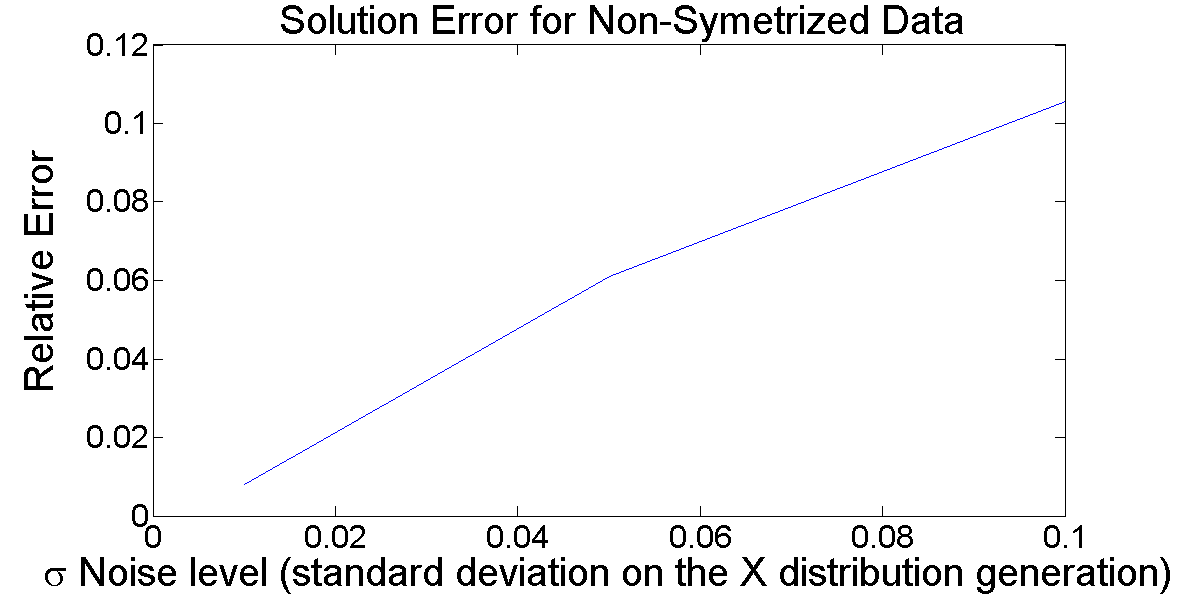
\includegraphics[width=3.3in]{figure/normerror}
\centering
\caption{Performance of the Batch Method at Various Noise Levels}
\label{normerror}
\end{figure}

\begin{figure}[h]
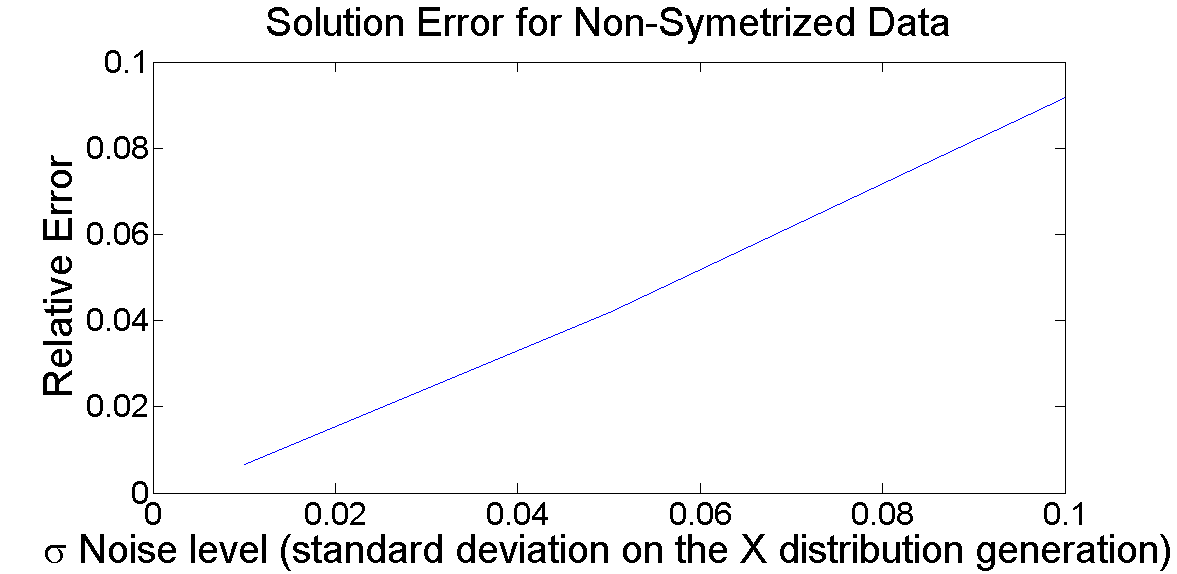
\includegraphics[width=3.3in]{figure/normerrorsym}
\centering
\caption{Performance of the Batch Method at Various Noise Levels for Symmeterized Data}
\label{normerrorsym}
\end{figure}

It is observed that symmetrized data provides, to a degree, a better solution of $X$. Additionally, symmetrizing the data provides more $\{A, B\}$ pairs, which will become important for methods described in the following sections.

\section{THE EXPANDED BATCH METHOD (THE CASE OF NOISY A's)} \label{batchnoise}

When the sensor that generates $B=\{B_j\}$ is accurate and there is significant
measurement noise in the set $A = \{A_i\}$, a single $X$ will not solve every instance of Eq.(\ref{main}) and hence the delta function in Eq.(\ref{mainconvall}) 
will not solve the problem. Instead, we seek a distribution $f_X(H)$ with (a priori unknown) mean $M_X$ and covariance $\Sigma_X$.

We can re-write Eq.(\ref{main}) as
\begin{equation} A_i = X B_i X^{-1} \label{main2} \end{equation}
and in a similar fashion as in Eq.(\ref{mainconvall}),we can write the probabilistic form of Eq.(\ref{mainconvall}) as
\begin{equation} f_A(H) = (f_X * f_B* f_{X^{-1}})(H). \label{mainconvallwnoise2} \end{equation}

In the subsections that follow, we derive the conditions on the mean and covariance of $f_X$ and
develop numerical methods for solving for these quantities.

\subsection{Conditions on $M_X$ and $\Sigma_X$}
Using the associativity of convolution, $f_X * f_B* f_{X^{-1}} = f_X * (f_B* f_{X^{-1}})$, 
and applying Eq.(\ref{meancovconvdef}) to Eq.(\ref{mainconvallwnoise2}) twice, we get
\begin{equation}
\boxed{\,
M_A = M_X \, M_B \, M_{X^{-1}}
\,}
\label{covprop2} \end{equation}
and
\begin{equation}
\begin{split}
\Sigma_{A} = Ad(M_{X})[Ad(M_{B^{-1}}) \Sigma_{X} Ad^T(M_{B^{-1}}) + \Sigma_{B}]Ad^T(M_{X})\\
+ \Sigma_{X^{-1}}.
\end{split}
\label{covprop22}
\end{equation}
Note that Eq.(\ref{covprop2}) and Eq.(\ref{covprop22}) are built on the use of (\ref{meancovconvdef}) twice so that they are approximations, unlike
Eq.(\ref{mainmain11}) and Eq.(\ref{mainmain12}) which are exact (by Theorem \ref{exactthm}). 
We can simplify this relationship in Eq.(\ref{covprop22}) by proving two identities related to the mean and 
covariance of probability distributions on $SE(3)$ given below.

As in the noise-free case, $(M_A,\Sigma_A)$ and $(M_B,\Sigma_B)$ are known from the data and are computed from
Eq.(\ref{datameancovconvdef}). The only difference is that now we seek $(M_X, \Sigma_X)$ instead of just $X$.

With these two properties, as well as the fact that $[Ad(H)]^{-1}=Ad(H^{-1})$, we can write Eq.(\ref{covprop22}) as:
\begin{flalign*}
\Sigma_A = &Ad(M_X) \, Ad(M_B^{-1}) \, \Sigma_{X} \, Ad^T(M_B^{-1}) \, Ad^T(M_X)\\
&+ Ad(M_X) \, \Sigma_{B} \, Ad^T(M_X) + Ad(M_X) \, \Sigma_{X}\, Ad^T(M_X), 
\end{flalign*}
or equivalently 
\begin{flalign*}
&Ad(M_X^{-1}) \, \Sigma_A \, Ad^T(M_X^{-1}) =\\
&Ad(M_B^{-1}) \, \Sigma_{X} \, Ad^T(M_B^{-1}) + \Sigma_{B} + \Sigma_{X}, 
\end{flalign*}
which leads to our final result 
\begin{equation}
\boxed{\,
\begin{split}
&\Sigma_{X} + Ad(M_B^{-1}) \, \Sigma_{X} \, Ad^T(M_B^{-1}) =\\
&Ad(M_X^{-1}) \, \Sigma_A \, Ad^T(M_X^{-1}) - \Sigma_{B}.
\end{split}
\,}
\label{covprop1112} \end{equation}
As in the noise-free case, $(A,\Sigma_A)$ and $(B,\Sigma_B)$ are known from the data and are computed from
Eq.(\ref{datameancovconvdef}). The only difference is that now we seek $(M_X, \Sigma_X)$ instead of just $X$.

\subsection{Computing $M_X$ and $\Sigma_X$}
From Eq.(\ref{covprop1112}), we can solve for $\Sigma_X$, given an $M_X$. This is done by taking the Kronecker product of both sides and writing
\begin{equation}
\begin{split}
[&Ad(M_B^{-1}) \otimes Ad(M_B^{-1}) + \mathbb{I}_{36}] {\rm vec}(\Sigma_X)\\
&= {\rm vec}(Ad(M_X^{-1}) \Sigma_{A} Ad^T(M_X^{-1}) - \Sigma_{B}),
\end{split}
\label{kroncovprop1112} \end{equation}
from which we obtain ${\rm vec}(\Sigma_X)$, and hence $\Sigma_X$.
Since $[Ad(M_B^{-1}) \otimes Ad(M_B^{-1}) + \mathbb{I}_6 \otimes  \mathbb{I}_6]$ in general will be non-singular, there is an exact solution of $\Sigma_X$ for every given $M_X$. This unique value of $\Sigma_X$ indicates the variation of $X$s, about the mean ($M_X$), needed to relate the sets of noisy data ($A$'s and $B$'s) in the $A_i=X_iB_iX_i^{-1}$ relationship. $\Sigma_X$ then becomes very useful for quantifying the``correctness" of a $M_X$. $\Sigma_{X_{calc}}$ is composed of the following variances on the values from the 6-dimensional Lie algebra,
\begin{equation}
\Sigma_{X_{calc}}=\left(
\begin{array}{cccccc}
\sigma_{\omega_1}^2 & \sigma_{\omega_1\omega_2} & \sigma_{\omega_1\omega_3} & \sigma_{\omega_1v_1} & \sigma_{\omega_1v_2} & \sigma_{\omega_1v_3}\\
\sigma_{\omega_2\omega_1} & \sigma_{\omega_2}^2 &\sigma_{\omega_2\omega_3} & \sigma_{\omega_2v_1} & \sigma_{\omega_2v_3} & \sigma_{\omega_2v_3}\\
\sigma_{\omega_3\omega_1} & \sigma_{\omega_3\omega_2} & \sigma_{\omega_3}^2 & \sigma_{\omega_3v_1} & \sigma_{\omega_3v_2} & \sigma_{\omega_3v_3}\\
\sigma_{v_1\omega_1} & \sigma_{v_1\omega_2} & \sigma_{v_1\omega_3} & \sigma_{v_1}^2 & \sigma_{v_1v_2} & \sigma_{v_1v_3}\\
\sigma_{v_2 \omega_1} & \sigma_{v_2 \omega_2} & \sigma_{v_2 \omega_3} & \sigma_{v_2 v_1} & \sigma_{v_2}^2 & \sigma_{v_2 v_3}\\
\sigma_{v_3 \omega_1} & \sigma_{v_3\omega_2} & \sigma_{v_3\omega_3} & \sigma_{v_3 v_1} & \sigma_{v_3 v_2} & \sigma_{v_3}^2\\
\end{array}\right).
\end{equation}
The information contained in $\Sigma_{X_{calc}}$ could be used to find the most favorable (least uncertainty in $X_{calc}$) directions for planning trajectories, sensor placement or other pose dependent tasks.

\subsection{Numerical Validation of $\Sigma_X$}
To verify that this formulation produced a meaningful $\Sigma_X$, we used a numerical approach that would allow us to, a prioir, know the true distribution of $X$. We simulate an $AX=XB$ calibration by generating simulated $A$ and $B$ data streams. The $B$s are chosen as poses along a trajectory in $SE(3)$. Since we must use relative motions, we generate $B^{ij}=B_i^{-1}B_{i+1}$ where $B_i$s are drawn from the two sample``s-shaped" trajectories on a sphere. After forming relative motions, $B_{ij}$'s, we calculate $A^{ij}= ^1\hspace{-0.05in}X_{ij}\,\,B_i\,\,^2X_{ij}^{-1}$, where $^1X_{ij}$ and $^2X_{ij}$ are drawn from a distribution with known mean ($X$) and covariance. Each calculation of $^kX_{ij}$ is tweaked as such:
\begin{equation} ^kX_{ij} \,\doteq\, X \,\, ^k\Delta_{ij} \label{noisybdef} \end{equation}
where $^k\Delta_{ij}$ is a matrix of small noises of the the form
$$ ^k\Delta_i \doteq
\exp \left(
\begin{array}{ccc}
\Omega (\delta t) & & {\bf v} (\delta t) \\ \\
{\bf 0}^T & & 0 \end{array}
\right) \,
\approx \, \mathbb{I}_4 + (\delta t) \left(
\begin{array}{ccc}
\Omega & & {\bf v} \\ \\
{\bf 0}^T & & 0 \end{array}
\right). $$
where $\Omega = - \Omega^T$ and ${\bf v}$ are random angular and translational velocities with components drawn independently from
a Gaussian distribution with variance $\sigma^2$, and $\delta t$ is a small finite time.

After calculating $\Sigma_X$ from Eq.($\ref{covprop1112}$), we can compare the calculated sample mean and covariance of $\{X_{ij}\}=\{^1X_{ij}\} \cup \{^2X_{ij}\}$ with the solved for values.


\begin{figure}[h]
\begin{center}
\setlength{\unitlength}{0.012500in}%
 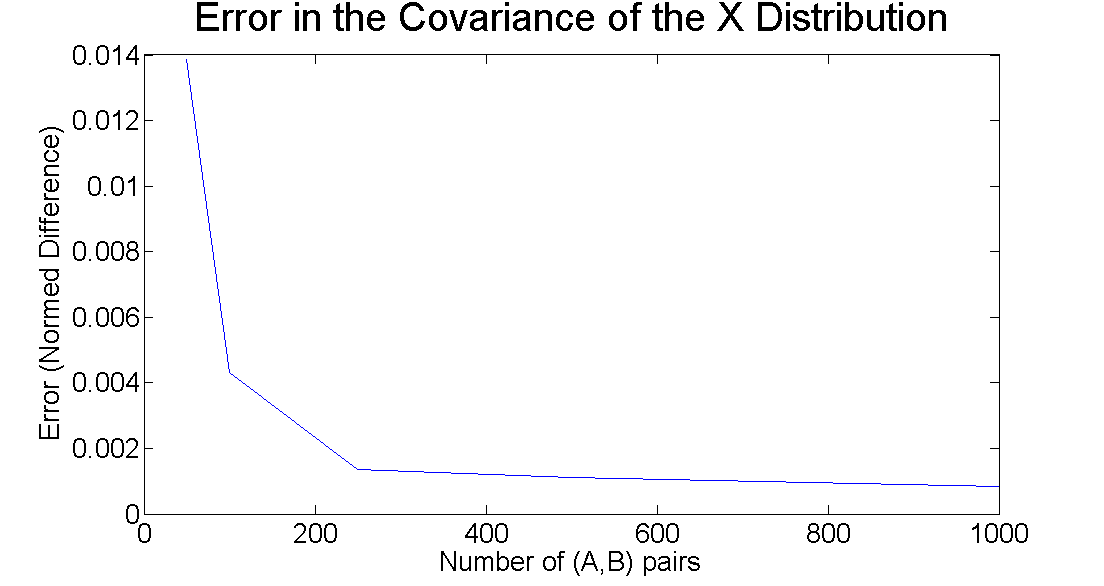
\includegraphics[width=3.3in]{figure/sigerror}
\end{center}
\caption{The Above Plot Shows that the $\Sigma_X$ is Calculated from ($\ref{covprop1112}$) and Becomes More Accurate as the Number of Data Samples Increases}
\label{figure_ASME} 
\end{figure}


\section{Relating the Covariances of a PDF and Its Symmetrized Version}

Recall that given an arbitrary pdf $f(H)$ with mean $M$ and covariance $\Sigma$, a symmetrized version is defined as:
$$ \tilde{f}(H) = \half ({f}(H) + {f}(H^{-1}) ). $$
Let $\tilde{M}$ and $\tilde{\Sigma}$ denote the mean and covariance of $\tilde{f}(H)$. 
Given that symmetrization of a pdf puts the mean of the result at the identity, we already know that $\tilde{M} = \mathbb{I}$.
The remaining question to ask is what the relationship is between the covariances of the original and symmetrized versions of a pdf.
This is answered here.

From the definition of covariance and the invariance of the integral over $SE(3)$ under inversions, and the fact that $\tilde{M} = \mathbb{I}$, the following equation
$$ \tilde{\Sigma} = \int_{SE(3)} \log^{\vee}(H)  [\log^{\vee}(H)]^T \tilde{f}(H) dH $$
can be simplified as:
$$ \tilde{\Sigma} = \int_{SE(3)} \log^{\vee}(H)  [\log^{\vee}(H)]^T {f}(H) dH. $$
This is not to be confused with
$$ {\Sigma} = \int_{SE(3)} \log^{\vee}(M^{-1} H)  [\log^{\vee}(M^{-1} H)]^T {f}(H) dH. $$
where
$$ \int_{SE(3)} \log^{\vee}(M^{-1} H)  {f}(H) dH = \mathbb{O}. $$

Though there appears to be no simple exact relationship between $\tilde{\Sigma}$ and ${\Sigma}$, in the case when $\|\Sigma\|$ and $\|M\|$ are both reasonably
small, an approximate relationship can be constructed by using the Baker-Campbell-Hausdorf formula to expand out $\log^{\vee}(M^{-1} H)$. 
This was done in \cite{wang06}, and the result (modulo different notation) is:
\begin{equation}
\tilde{\Sigma} = \Sigma + (\log^{\vee} M)(\log^{\vee} M)^T + \half \left(\Sigma \, ad^T(\log M) + ad(\log M) \, \Sigma\right)
\label{sigtildesig}
\end{equation}
If $(M,{\Sigma})$ is known a priori, then $\tilde{\Sigma}$ can be computed from them. Due to the simple computation of $\tilde{\Sigma}$, Eq.(\ref{sigtildesig}) can be used as a consistency
check on the accuracy of $M$ and $\Sigma$ by computing the norm of the difference of both sides.
\end{comment}


\section{CONCLUSION AND FUTURE WORK}
In this paper we rexamined the ``AX=XB'' formulation of the sensor calibration problem used in camera calibration, Cartesian robot hand calibration, robot eye-to-hand calibration, aerial vehicle sensor calibration and image guided therapy (IGT) sensor calibration. A summary of some of the most influential and effective previous methods was presented and their positive and negative traits were discussed. We focused on the case where there is noise on the incoming sensor data, and therefore multiple sensor readings are needed. It was clear that each algorithm has strengths in different contexts and problems and it is important to use the appropriate method for the circumstance.\\
In addition to measurement error contributing to noise, we emphasized the fact that the sensor data streams containing the $A$s and $B$s may present at different sample rates, be asynchronous, and each stream may contain gaps in information. We therefore presented a method for calculating the calibration transformation that works for data without any a priori knowledge of the correspondence between the $A$s and $B$s. The new method formulates the sensor data as probability distributions and gives the mean solution, $X_{calc}$. Additionally, we show how the covariance of $X_{calc}$ can be determined which could give insight into the magnitude and type of noise on the sensor measurements.\\
In future works, we would like to continue to examine, in more detail, the usefulness of $\Sigma_X$. We will further explore the relationship between the $X$ covariance and the error on the calibration in experimental results, hypothetically using $\Sigma_X$ to identify ideal sensor placements in the environment and path plan along minimal error regions. Additionally, we hope to harness the knowledge of $\Sigma_X$ to formulate a cost function for minimizing the error on our initial solution.




%%%%%%%%%%%%%%%%%%%%%%%%%%%%%%%%%%%%%%%%%%%%%%%%%%%%%%%%%%%%%%%%%%%%%%
\begin{acknowledgment}
The authors would like to recognize NSF Grant RI-Medium: IIS-1162095, which served to support this work. We would also like to acknowledge the support of Alexis Cheng and Emad M. Boctor, colleagues in this endeavor at Johns Hopkins University.
\end{acknowledgment}



%
%%%%%%%%%%%%%%%%%%%%%%%%%%%%%%%%%%%%%%%%%%%%%%%%%%%%%%%%%%%%%%%%%%%%%%%
\appendix       %%% starting appendix
\section*{Appendix A: Integration and Convolution on SE(3)}

This appendix reviews those features of integration and convolution on the group $SE(3)$ that are
relevant to the formulation in this paper. For more detailed treatments see \cite{myoldbook, vol2}.

\subsection*{Integration}

$SE(3)$ is a six-dimensional matrix Lie group. If $H = H({\bf q})$ where ${\bf q} = [q_1,....,q_6]^T$ is a global set of coordinates, then
functions $f:SE(3) \rightarrow \mathbb{R}$ can be integrated as
$$ \int_{SE(3)} f(H) dH \doteq \int_{{\bf q} \in D} f(H({\bf q})) |J({\bf q})| d{\bf q} $$
where $D$ is the domain of integration in parameter space and $d{\bf q} = dq_1 dq_2 \cdots dq_6$. 
The Jacobian determinant $|J({\bf q})|$ is computed from the Jacobian matrix 
$$ J({\bf q}) = \left[\left(H^{-1} \frac{\partial H}{\partial q_1}\right)^{\vee}; \left(H^{-1} \frac{\partial H}{\partial q_2}\right)^{\vee};\,\cdots\,
\left(H^{-1} \frac{\partial H}{\partial q_6}\right)^{\vee}\right]. $$
For example, if Cartesian coordinates are used for the translation vector and $ZXZ$ Euler angles are used
for rotations, then ${\bf q} = [x,y,z,\alpha,\beta,\gamma]^T$, $D=\mathbb{R}\times\mathbb{R}\times\mathbb{R}\times[0,2\pi]\times[0,\pi]\times[0,2\pi]$ and $J({\bf q}) = \sin \beta$. And while $D$ and $J({\bf q})$ will change depending on what parameterization is used, the value of the integral itself does not, as it is a property of the
Lie group and the function, and not how the function is expressed and the integral is computed in coordinates.

$SE(3)$ is unimodular, which means that the integation measure, $dH = |J({\bf q})| d{\bf q}$, has the property that for any
fixed $H_0 \in SE(3)$ and ``well behaved fuction\footnote{Here we mean a function for which the integral exists, and hence
$f \in L^1(SE(3))$, and later that the convolution integral exists, which is guaranteed by further requiring that
$f \in L^2(SE(3))$. And so, with the notable exception of the Dirac delta function, we restrict the discussion to
$f \in (L^1 \cap L^2)(SE(3))$.}'' $f:SE(3) \rightarrow \mathbb{R}$, \cite{myoldbook}
\begin{equation}
\int_{SE(3)} f(H_0 \circ H) dH = \int_{SE(3)} f(H \circ H_0) dH = \int_{SE(3)} f(H) dH.
\label{defuni}
\end{equation}
In addition, it can be shown that when these conditions hold, so too does
\begin{equation}
\int_{SE(3)} f(H^{-1}) dH = \int_{SE(3)} f(H) dH.
\label{invdsdcf}
\end{equation}
A common source of confusion is that many books on Lie groups are concerned with compact Lie groups, which possess both bi-invariant metrics
and bi-invariant integration measures. When going to the noncompact case, bi-invariant metrics generally do not exist (except for special cases
such as products of tori and Euclidean spaces), and they do not exist for $SE(3)$. Though bi-invariant integration measures also do not exist in general,
they do exist for a broader class of special noncompact Lie groups than those that have bi-invariant metrics, and this includes $SE(3)$. 

\subsection*{Convolution} \label{convsec}

Given two functions, $f_1, f_2 \in (L^1 \cap L^2)(SE(3))$, the convolution is defined as
\begin{equation}
(f_1 * f_2)(H) \doteq \int_{SE(3)} f_1(K) f_2(K^{-1} H) dK. 
\label{convdef}
\end{equation}
This integral can be rewitten in a number of equivalent forms using Eq.(\ref{defuni}) and Eq.(\ref{invdsdcf}).
Convolution inherits the associative property from the underlying group, which is written as 
$$ (f_1 * f_2) * f_3 = f_1 * (f_2 * f_3) $$
(where the dependence of these functions on $H$ has been temporarily suppressed). In analogy with the way it inherit associativity, convolution 
also inherits noncommutativity for general functions, with the exception of special functions called ``class functions''.

If we expand the class of functions that are considered beyond $(L^1 \cap L^2)(SE(3)$
to include Dirac delta functions\footnote{As in $\mathbb{R}^n$, these can be thought of as spikes
of infinite height and infinitesimal width centered on the identity}, which are the unique functions such that for every $f \in (L^1 \cap L^2)(SE(3)$
$$ (f * \delta)(H) = (\delta * f)(H) = f(H), $$
then the result is the ``group algebra'' consisting of functions as elements, and the two operations of convolution and addition of
functions: $f_1*f_2$ and $f_1 + f_2$. A slightly further expansion of allowable functions to include shifted delta functions of the form:
$$ \delta_X(H) \doteq \delta(X^{-1} H) = \delta( H X^{-1}). $$
The unshifted delta function is an example of a symmetric function, in that $\delta(H) = \delta(H^{-1})$.

Using the properties of the invariant integral on $SE(3)$, convolving a shifted delta function with an arbitrary
function transfers the shift:
\begin{equation}
\begin{split}
(\delta_X * f)(H) =& \int_{SE(3)} \delta(X^{-1} K) f(K^{-1} H) dK \\
=& \int_{SE(3)} \delta(J) f((XJ)^{-1} H) d{\color{red}K} = f(X^{-1} H) \\
\end{split}
\end{equation}
where the change of variables $J = X^{-1} K$ and the invariance of integration have been used.
Similarly,
$$ (\delta_X * f * \delta_{X^{-1}})(H) = f(X^{-1} H X). $$
Using the associative property,
\begin{equation}
\begin{split}
&(\delta_X * f_1 * \delta_{X^{-1}}) * (\delta_X * f_2 * \delta_{X^{-1}}) \\
&= \delta_X * f_1 * (\delta_{X^{-1}} * \delta_X) * f_2 * \delta_{X^{-1}} \\ 
&= \delta_X * (f_1 * f_2)* \delta_{X^{-1}}. 
\end{split}
\end{equation}

\begin{comment}
\subsection*{Symmetric Functions and Class Functions}

A symmetric function is one with the property that
$$ s(H) = s(H^{-1}). $$
There are several ways to construct symmetric pdfs from nonsymmetric ones. For example, if $f$ is a pdf, 
$\tilde{f}(H) = \half(f(H) + f(H^{-1})$ is symmetric (with the factor of $1/2$ necessary to make the result a pdf).
$f(H)\cdot f(H^{-1})/((f*f)(\mathbb{I}))$ is also symmetric and normalized to be a pdf (where $\cdot$ is just scalar
multiplication of functions). Also, if $f(H)$ is an arbitrary pdf and $f'(H) = f(H^{-1})$, then $(f*f')(H)$ will be symmetric.

Using the invariance properties of the integral over $SE(3)$, it is not difficult to see that 
\begin{eqnarray*}
(s_1 * s_2)(H) &=& \int_{SE(3)} s_1(K) s_2(K^{-1} H) dK \\
&=& \int_{SE(3)} s_1(K^{-1}) s_2(H^{-1} K) dK. \end{eqnarray*}
Then changing variables as $J = H^{-1} K$, $HJ =K$, and $K^{-1} = J^{-1} H^{-1}$ so
$$ (s_1 * s_2)(H) = \int_{SE(3)} s_2(J) s_1(J^{-1} H^{-1}) dJ = (s_2 * s_1)(H^{-1}). $$
This is not the same as saying that the convolution of two symmetric functions is symmetric. Nor does it say that
the convolution of symmetric functions is commutative. But, it does say that
the convolution of a symmetric function with itself is symmetric. 

In general, the only functions on a group that commute under convolution with every function are the class functions.
A class function has the property that
$$ \chi(K H K^{-1}) = \chi(H) $$
for every $H,K$ in the group. For example, $\delta$ is a class function for $SE(3)$, and the fact that it commutes under
convolution was already explained in (\ref{convsec}).
\end{comment}

% Here we show that in general class function commute under convolution.
%
%*** will fill if needed. may not be very relevant ***
%
%Unfortunately, no class functions on $SE(3)$ are in $(L^1 \cap L^2)(SE(3))$.


%%%%%%%%%%%%%%%%%%%%%%%%%%%%%%%%%%%%%%%%%%%%%%%%%%%%%%%%%%%%%%%%%%%%%%%
%\section*{Appendix B: Head of Second Appendix}
%\subsection*{Subsection head in appendix}
%The equation counter is not reset in an appendix and the numbers will
%follow one continual sequence from the beginning of the article to the very end as shown in the following example.
%\begin{equation}
%a = b + c.
%\end{equation}


%%%%%%%%%%%%%%%%%%%%%%%%%%%%%%%%%%%%%%%%%%%%%%%%%%%%%%%%%%%%%%%%%%%%%%
% The bibliography is stored in an external database file
% in the BibTeX format (file_name.bib).  The bibliography is
% created by the following command and it will appear in this
% position in the document. You may, of course, create your
% own bibliography by using thebibliography environment as in
%
% \begin{thebibliography}{12}
% ...
% \bibitem{itemreference} D. E. Knudsen.
% {\em 1966 World Bnus Almanac.}
% {Permafrost Press, Novosibirsk.}
% ...
% \end{thebibliography}

% Here's where you specify the bibliography style file.
% The full file name for the bibliography style file 
% used for an ASME paper is asmems4.bst.
\bibliographystyle{asmems4}

% Here's where you specify the bibliography database file.
% The full file name of the bibliography database for this
% article is asme2e.bib. The name for your database is up
% to you.
\bibliography{asme2e}
\end{document}









%%-------------------------------------------------------------------------------------
%\subsection{Solving for $X$ and $\Sigma_X$}
%
%
%
%
%\subsubsection{Gradient descent using the $L^2$ Norm}
%
%One possible method to search for an appropriate $X$ and $\Sigma_X$ could be by minimizing the cost function
%\begin{equation}
%C_2(X) = \left(\int_{SE(3)} \|f_1(H) - f_2(H)\|^2 \, dH \right)^{\half}.
%\label{cost2} \end{equation}
%where
%$$ f_1(H) = \rho(H; A, \Sigma_A) $$
%and
%\begin{equation}
%f_2(H) = \rho(H; X B X^{-1}, \,\, \Sigma_2).
%\end{equation}
%where
%$$ \Sigma_2 = Ad(X) [Ad(B^{-1})\Sigma_X Ad^T(B^{-1}) + \Sigma_{B} + \Sigma_X]Ad^T(X)$$
%In general, the integral in this cost function cannot be solved in closed form because the $\log$ function is nonlinear, and in terms of exponential coordinates
%$dH = |J({\bf z})| d{\bf z}$ where $|J({\bf 0})| =1$, but this Jacobian is a nonlinear function of ${\bf z}$.
%
%However, if we a priori limit the search for $X$ to the cylinder
%defined in (\ref{cylinder}), automatically, $X B X^{-1} = A$.
%Then, we can define a new variable $K = M_A^{-1} H$ and using the property of
%invariance of integration under shifts, can write
%$$ C_2(X(\phi,s), \Sigma_X) = \left(\int_{SE(3)} \left| f'_A(K) - f'_B(K) \right|^2 \, dK \right)^{\half} $$
%where
%$$ f'_1(K) = \rho(K; \mathbb{I}_4, \Sigma_A) $$
%and
%$$  f'_2(K) = \rho(K;\mathbb{I}_4 \,,\, \Sigma_2).$$
%where
%\begin{equation}
%\begin{split}
%\Sigma_2= &Ad(X(\phi,s)) [Ad(B^{-1})\Sigma_{X(\phi,s)} Ad^T(B^{-1})\\
%&+ \Sigma_{B} + \Sigma_X(\phi,s)]Ad^T(X(\phi,s))
%\end{split}
%\end{equation}
%And if covariances are scaled to be small, the benefit of this is that it reduces to the integral of the norm of the difference of two Gaussians.
%This has a closed-form solution
%\begin{equation}
%\begin{split}
%C_2(X(\phi,s), \Sigma_X) = (2\pi)^{-3}&\left[ -2 \frac{\sqrt{\| \Sigma_2^{-1} + \Sigma_A^{-1} \|^{-1}}}{\sqrt{\| \Sigma_A \|}\sqrt{\| \Sigma_2 \|}}\right.\\
%&\left. + \frac{\sqrt{\| \Sigma_2 \|}}{\sqrt{2}\| \Sigma_2 \|} + \frac{\sqrt{\| \Sigma_A \|}}{\sqrt{2}\| \Sigma_A\|} \right]
%\end{split}
%\end{equation}
%which can be minimized by a search over the 2 remaining DOF of $X$ and the 21 unique entries of $\Sigma_X$.
%
%In a similar manner, we can write another cost function, derived from the Kullback–Leibler divergence, and find the global minimum of the cost function
%\begin{equation}
%C_2(X) = D_{KL}(f_A \,\|\, \delta_X * f_B  * \delta_{X^{-1}})
%\label{cost3} \end{equation}
%where $f_A(H) = \rho(H; M_A, \Sigma_A)$ and
%$$ (\delta_X * f_B  * \delta_{X^{-1}})(H) = \rho(H;\, X M_B X^{-1} \,,\, Ad(X) \,\Sigma_{B}\, Ad^T(X)). $$
%
%As before, if we limit the search for $X$ to the cylinder, the KL divergence of
%two distributions on $\mathbb{R}^n$ with means ${\bf m}_i$ and covariances $\Sigma_i$ is
%$$ D_{KL}(f_1 \,\|\, f_2) = $$
%$$ \half\left[{\rm tr}(\Sigma_2^{-1} \Sigma_1) + ({\bf m}_2 - {\bf m}_1)^T \Sigma_2^{-1} ({\bf m}_2 - {\bf m}_1)
%-n - {\rm ln}\left(\frac{|\Sigma_1|}{|\Sigma_2|}\right)\right]. $$
%%% The above is from Wikipedia http://en.wikipedia.org/wiki/Kullback%E2%80%93Leibler_divergence
%In our problem, ${\bf m}_2 - {\bf m}_1 = {\bf 0}$, and since $SE(3)$ is
%unimodular, $|Ad(X)| = 1$. 
%Our cost function then becomes
%$$ C_2(X(\phi,s), \Sigma_X) = D_{KL}(f'_A \,\|\, f'_B) $$
%where
%$$ C'_2(X(\phi,s), \Sigma_X) = {\rm tr}(\Sigma_A^{-1} \Sigma_2) - {\rm ln} \left( \frac{| \Sigma_A |}{|\Sigma_2|} \right), $$
%and we minimize over the 23 parameters.
%
%
%
%
%\subsubsection{Block decomposition}
%
%As in the no noise case, we can obtain the rotational component, $R_X$, of $X$. From (\ref{covprop2}) we have that,
%\begin{equation}
%{\bf n}_{A}=R_X{\bf n}_{B}
%\label{ns}\end{equation}.\\
%
%If we decompose $\Sigma_{A}$ and $\Sigma_{B}$ into blocks as
%$ \Sigma_{i}= \left(\begin{array}{cc}
%\Sigma_{i}^1 & \Sigma_{i}^2 \\
%\Sigma_{i}^3 & \Sigma_{i}^4  \end{array}\right) $\\
%\\
%where $\Sigma_{i}^3 = (\Sigma_{i}^2)^T$, then we can take (\ref{covprop1112})
%$$\Sigma_{X} + Ad(B^{-1}) \Sigma_{X} Ad^T(B^{-1}) = Ad(X^{-1}) \Sigma_A Ad^T(X^{-1}) - \Sigma_{B}$$
%and write
%\begin{equation}
%\begin{split}
%&\left[\begin{array}{cc}
%\Sigma_{X}^1 &\Sigma_{X}^2 \\
%\Sigma_{X}^3 & \Sigma_{X}^4  \end{array}\right]+
%\left[\begin{array}{cc}
%R_{B}^T &  0 \\
%(\widehat{-R_{B}^Tt_B})R_{B}^T &R_{B}^T \end{array}\right]
%\left[\begin{array}{cc}
%\Sigma_{X}^1 &\Sigma_{X}^2 \\
%\Sigma_{X}^3 & \Sigma_{X}^4  \end{array}\right]
%\left[\begin{array}{cc}
%R_{B} &  R_{B}(\widehat{R_{B}^Tt_B}) \\
%0 &R_{B} \end{array}\right]=\\
%&\left[\begin{array}{cc}
%R_{X}^T &  0 \\
%(\widehat{-R_{X}^Tt_X})R_{X}^T &R_{X}^T \end{array}\right]
%\left[\begin{array}{cc}
%\Sigma_{A}^1 &\Sigma_{A}^2 \\
%\Sigma_{A}^3 & \Sigma_{A}^4  \end{array}\right]
%\left[\begin{array}{cc}
%R_{X} &  R_{X}(\widehat{R_{X}^Tt_X}) \\
%0 &R_{X} \end{array}\right]-
%\left[\begin{array}{cc}
%\Sigma_{B}^1 &\Sigma_{B}^2 \\
%\Sigma_{B}^3 & \Sigma_{B}^4  \end{array}\right].
%\end{split}
%\end{equation}
%Given that
%\begin{equation}
%\begin{split}
%&\left[\begin{array}{cc}
%R^T &  0 \\
%(\widehat{-R^Tt})R^T & R^T \end{array}\right]
%\left[\begin{array}{cc}
%\Sigma^1 &\Sigma^2 \\
%\Sigma^3 & \Sigma^4  \end{array}\right]
%\left[\begin{array}{cc}
%R &  R(\widehat{R^Tt}) \\
%0 &R \end{array}\right]=\\
%&\left[\begin{array}{cc}
%R^T \Sigma^1 R &  R^T \Sigma^1 R (\widehat{R^Tt}) +R^T \Sigma^2 R \vspace{0.1in}\\
%\multirow{2}{*}{$(\widehat{-R^Tt})R^T \Sigma^1 R + R^T \Sigma^3 R$} & (\widehat{-R^Tt})R^T \Sigma^1 R (\widehat{R^Tt})+ R^T \Sigma^3 R (\widehat{R^Tt}) \\
% &+ (\widehat{-R^Tt}) R^T \Sigma^2 R + R^T \Sigma^4 R \end{array}\right]
%\end{split}
%\end{equation}
%we can write the block equations as:
%\begin{align} 
%&\Sigma_X^1 + R_B^T \Sigma_X^1 R_B =  R^T_X \Sigma_A^1 R_X - \Sigma_B^1\\
%\nonumber&\Sigma_X^2 + R_B^T \Sigma_X^1 R_B (\widehat{R_B^Tt_B}) + R_B^T \Sigma_X^2 R_B\\ 
%&=  R^T_X \Sigma_A^1 R_X (\widehat{R_X^Tt_X}) +R_X^T \Sigma_A^2 R_X - \Sigma_B^2 \\
%\nonumber &\Sigma_X^3 + (\widehat{-R_B^Tt_B}) R_B^T \Sigma_X^1 R_B + R_B^T \Sigma_X^3 R_B\\
%&=  (\widehat{-R_X^Tt_X}) R^T_X \Sigma_A^1 R_X + R_X^T \Sigma_A^3 R_X - \Sigma_B^3 \\
%\begin{split}& \Sigma_X^4 + (\widehat{-R_B^Tt_B}) R_B^T \Sigma_X^1 R_B (\widehat{R_B^Tt_B})  + R_B^T \Sigma_X^3 R_B (\widehat{R_B^Tt_B})\\ 
%&+ (\widehat{-R_B^Tt_B}) R_B^T \Sigma_X^2 R_B + R_B^T \Sigma_X^4 R_B = \\
%&(\widehat{-R_X^Tt_X}) R_X^T \Sigma_A^1 R_X (\widehat{R_X^Tt_X}) \\
%&+ R_X^T \Sigma_A^3 R_X (\widehat{R_X^Tt_X}) + (\widehat{-R_X^Tt_X}) R_X^T \Sigma_A^2 R_X + R_X^T \Sigma_A^4 R_X - \Sigma_B^4 \end{split}
%\end{align}
%%--------------------------
